\documentclass[pdflatex,sn-basic]{sn-jnl}
\usepackage{graphicx}
\usepackage{amsmath,amssymb,amsfonts}
\usepackage{booktabs}
\usepackage{longtable}
\usepackage{longtable}
\usepackage{longtable}
\usepackage{longtable}
\usepackage{longtable}
\usepackage{longtable}

\raggedbottom

\begin{document}

\title[Trustworthy AI for Low-Carbon Geopolymers]{From Property Prediction to Clean-Technology Deployment: A Systematic Review and Roadmap for Trustworthy AI in Low-Carbon Geopolymer Development}

\author*[1]{\fnm{Vinoth} \sur{Nageshwaran}}\email{vnageshwaran41452@ucumberlands.edu}
\author[2]{\fnm{Pooja} \sur{Bhardwaj (Chaggar)}}
\author[3]{\fnm{Sudhir S.} \sur{Amritphale}}

\affil*[1]{\orgname{University of the Cumberlands}, \orgaddress{\city{Williamsburg}, \state{KY}, \country{USA}}}
\affil[2]{\orgname{Western Sydney University}, \orgaddress{\city{Kingswood}, \state{NSW}, \country{Australia}}}
\affil[3]{\orgname{Science Investments LLC (formerly Louisiana Tech University)}, \orgaddress{\city{Ruston}, \state{LA}, \country{USA}}}

\abstract{Geopolymers synthesized from industrial residues are among the most credible low-carbon alternatives to Portland cement, and artificial intelligence (AI) is widely claimed to accelerate their development. This review audits that claim: has AI-enabled geopolymer research progressed from isolated property prediction toward trustworthy, physics-aware, environmentally quantified, and deployable clean-material design? Following PRISMA 2020, 894 unique records were identified; 729 were included, resolving to 677 unique primary studies (2013--2026), 71\% postdating the closest prior review, dual-screened in a primary + 1 design (kappa = 0.83/0.69). Every study was coded on a six-axis taxonomy, a trustworthy-AI scorecard, a five-level physics-integration audit, and an environmental-evidence ladder; coding reliability was verified by two independent blind recodes (one human, one procedural), with criterion-sensitive figures stated as bounds. Prediction and optimization constitute 95.7\% of the corpus, with demonstrated design-space search at roughly 10--17\%; adaptive experimentation comprises three simulated demonstrations; the autonomous stage is empty. Explainability has diffused widely (29.1\% of studies), but calibration (1.3\%), external validation (4.0\%), and reproducible artifacts (below 1\%) have not. Half of all physics-informed claims (14 of 27) deflate under audit, above a frontier of nine verified studies (1.3\%). Nearly half of this sustainability-framed literature quantifies no environmental variable; ISO-consistent life-cycle assessment appears in roughly 0.3\% of studies. Nine evidence-based gaps with acceptance criteria anchor a staged roadmap --- honest models, then chemistry- and carbon-coupled models, then closed loops, with deployment and governance in parallel. The coded corpus, audit tables, and scripts are released as open, DOI-archived infrastructure.}

\keywords{geopolymer, alkali-activated materials, machine learning, trustworthy AI, life-cycle assessment, low-carbon construction}

\maketitle

\section{Introduction}

Cement production emits on the order of seven to eight percent of anthropogenic CO$_2$, and the demand curve for concrete bends upward through mid-century. Among the credible substitutes, geopolymers and alkali-activated materials (AAMs) occupy a distinctive position: they promise not only a large reduction in embodied carbon relative to Portland systems but the valorization of the industrial residues --- fly ash, slags, red mud, mine tailings --- whose disposal is itself an environmental liability. Their obstacle is equally distinctive. AAMs are not one material but a combinatorial family, synthesized from heterogeneous, regionally variable feedstocks under wide-ranging activation and curing regimes, so that the trial-and-error development which sufficed for a standardized commodity like Portland cement scales badly for them. This is precisely the kind of bottleneck artificial intelligence is claimed to relieve, and over the past decade a large literature has taken up the claim: machine-learned property prediction, explainable models, physics-informed learning, multi-objective and inverse design, and --- at least in prospect --- adaptive experimentation and autonomous discovery.

The premise of this review is that, for a clean-technology outcome, the interesting question is not whether AI can fit geopolymer data. It demonstrably can, hundreds of times over. The question is whether the field has progressed along the trajectory that would make those models \emph{matter}: from isolated property prediction toward models that are trustworthy (uncertainty-aware, calibrated, externally validated), physically and chemically grounded, environmentally quantified rather than environmentally rhetorical, adaptive rather than static, and ultimately connected to the acceptance frameworks through which construction materials actually reach practice. Each of these stages has an enthusiastic literature of claims; none has previously been audited. Prior reviews of AI in geopolymer research --- valuable as method catalogues and landscape surveys --- organize the field by algorithm or by predicted property, stop before the fastest-moving years, and do not interrogate trust, environmental quantification, or deployment at all (Section 4 and Table 1 position this review against them in detail).

This paper therefore undertakes a different kind of systematic review: an evaluative audit. From 894 uniquely identified records we assemble a frozen corpus of 729 included records representing 677 unique primary studies (2013--2026; Section 2.6) --- to our knowledge the largest yet analyzed at this intersection, with 71\% of it postdating the coverage window of the closest prior review --- and we subject it to instruments rather than summaries: a six-axis taxonomy coding every study's material system, task, trust profile, physics-integration level, environmental function, and deployment maturity; an eight-dimension trustworthy-AI scorecard; a five-level audit that grades physics and chemistry claims against what methods actually do; and an evidentiary ladder for environmental claims running from rhetoric to ISO-consistent life-cycle assessment. Three graded evidence levels --- demonstrated in geopolymers, demonstrated only in adjacent materials science, prospective --- discipline every capability claim, including our own.

The audit returns a coherent and uncomfortable picture, previewed here and developed in Sections 7--18. The field is 95.7\% prediction and optimization --- with demonstrated design-space search, as opposed to metaheuristically tuned prediction, estimated at roughly 10--17\% of the corpus by two independent recodes (Table S9) --- and its adaptive stage consists of three simulated demonstrations while its autonomous stage is empty. Explainability diffused rapidly (29.1\% of studies) while the trust practices that certify a model --- calibration (1.3\%), external validation (4.0\%), reproducible artifacts ($\sim$1\%) --- did not diffuse at all. Half of the field's physics-informed claims (14 of 27) deflate under audit, above a genuine but tiny frontier of nine verified studies (1.3\%) spanning thermodynamic hybrids, knowledge-guided designs, and constraint-embedded networks. And a literature framed almost universally around sustainability quantifies no environmental variable in 44.8\% of cases, performs ISO-grade life-cycle assessment in roughly 0.3\%, and optimizes carbon figures whose own uncertainty is never propagated. These are not counsels of despair; each deficiency is matched by demonstrated best practice \emph{inside the corpus}, which is what makes a roadmap credible rather than hortatory.

The review makes seven contributions. (1) The first systematic evidence base at the AI $\times$ geopolymer $\times$ clean-technology-deployment intersection, PRISMA-governed, with every record independently verified (primary + 1 dual-screening design, Section 2.3) and a released decision ledger. (2) A multidimensional taxonomy whose three views --- facets, maturity ladder, translation pipeline --- derive from one pre-registered coding. (3) A trustworthy-AI scorecard applied study-by-study, quantifying the explainability-without-reliability asymmetry. (4) A claimed-versus-verified audit of physics integration, with a reusable five-level scale. (5) An evidentiary grading of environmental claims culminating in the quantification pyramid. (6) An evidence-based gap framework (nine gaps, each with acceptance criteria) and a staged clean-technology roadmap whose logic --- honest models, then chemistry- and carbon-coupled models, then closed loops, with deployment and governance in parallel throughout --- follows from the gaps' dependency structure. (7) An open research artifact: the coded corpus, audit tables, and analysis scripts, released to serve as a seed for the community benchmark the field lacks.

The remainder of the paper proceeds as follows: methodology (Section 2); geopolymers as clean and circular technology for the general reader (Section 3); the field's evolution and prior reviews (Section 4); the taxonomy (Section 5); materials and data foundations (Section 6); then the synthesis ordered by the translation pipeline --- prediction (7), trust (8), physics (9), design (10), environmental assessment (11), waste valorization (12), twins and adaptive models (13--14) --- followed by the validation audit (15), deployment and governance (16--17), contradictions (18), gaps (19), roadmap (20), limitations of this review (21), and conclusions (22).

\section{Systematic Review Methodology}

\subsection{Protocol and reporting standard}

This review follows the PRISMA 2020 statement for systematic reviews. Because PROSPERO does not register materials-science reviews, the protocol --- research questions, eligibility criteria, screening design, coding schemes, and quality instruments --- was frozen in writing before search execution, and every subsequent deviation is disclosed as a dated amendment in this section. The review is organized around one evaluative question: to what extent has published AI-enabled geopolymer research progressed from isolated property prediction toward trustworthy, physics- and chemistry-aware, environmentally quantified, adaptive, and ultimately deployable clean-material design? Eight subsidiary research questions (RQ1--RQ8, Supplementary Table S1) operationalize this trajectory across materials and data, environmental performance, trustworthiness, physics integration, design capability, autonomy, and translation.

Two corpora are distinguished throughout. The \textbf{Core Corpus} contains primary peer-reviewed journal studies applying AI or machine learning to geopolymers or alkali-activated materials (AAMs) for construction-relevant purposes; it is governed by the PRISMA process and is the object of all quantitative synthesis. The \textbf{Context Corpus} contains prior reviews and adjacent-domain evidence (for example, self-driving-laboratory demonstrations in general materials science); it informs the maturity grading and roadmap but is never counted in PRISMA totals.

\subsection{Information sources and search}

Scopus served as the primary index. Six pre-registered query families targeted (A) the geopolymer $\times$ AI core, (B) trustworthy-AI terms, (C) physics- and chemistry-informed learning, (D) multi-objective and inverse design, (E) sustainability and carbon coupling, and (F) autonomous and agentic approaches, each restricted to English-language journal articles and reviews published from 2012 --- the year of the earliest identified ML--geopolymer study --- through August 2026. The Family-A core query, executed in Scopus advanced search on 10 August 2026, returned 774 records; Families B--F returned 403, 42, 123, 367, and 180 records respectively, the last feeding the Context Corpus. Verbatim query strings appear in Supplementary Table S2.

Scopus was complemented by three supplementary sources searched on the same date: ScienceDirect (title--abstract--keyword search, 320 records), the Crossref REST API (100 relevance-ranked records, capturing non-Elsevier venues), and SpringerLink (950 full-text matches identified; the top 20 relevance-ranked records were harvested at execution, and a random sample of 50 of the remaining 930 records was subsequently screened to bound the unharvested yield --- Section 21 reports the estimate). Families B--F served as coverage checks rather than an independent identification arm: their eligible hits were verified to be subsumed by the Family-A and supplementary harvests, and they contributed zero unique records to the screening pool (Figure 1, caption). IEEE Xplore was queried for completeness and returned 13 records, all conference papers and therefore ineligible; we report this as evidence that the computing literature holds no parallel journal corpus. Web of Science could not be searched because no Core Collection entitlement was available to the team; the multi-source design above mitigates, but does not eliminate, this coverage limitation. An initial fallback execution (ScienceDirect + Crossref + SpringerLink) preceded Scopus access by hours on the same day; both executions are retained in the audit trail, and all records were merged and deduplicated as described next.

\subsection{Study selection}

Records were deduplicated by DOI and normalized-title matching, with manual verification of near matches: of the 440 supplementary-source records (all counts post internal deduplication within each harvest), 320 matched Scopus records and were removed, leaving \textbf{894 unique records} (774 Scopus + 120 supplementary-only) for screening. Three further cross-source duplicates were detected and removed during screening itself, and a post-freeze duplicate-report audit during synthesis identified 52 more --- abbreviated-title twins that had escaped the merge; Section 2.6 describes their handling. Eligibility followed pre-registered criteria: inclusion required a peer-reviewed journal study applying AI/ML to geopolymers or AAMs --- including one-part systems, mortars, pastes, stabilized soils, and mine backfill --- for construction-relevant purposes, with heavy-metal solidification/stabilization and CO$_2$-capture composites explicitly retained. Exclusion codes covered preprints and non-journal items (EC1), out-of-scope materials (EC2), statistical-only studies without an ML method (EC3), conference proceedings (EC4), non-construction geopolymer functions such as adsorbents and catalysts (EC5), and duplicates (EC6). One criterion was added by dated amendment during adjudication (PRISMA 2020 item 24b): EC7 excludes venues not indexed in Scopus or Web of Science at screening date; it affected three records.

Screening proceeded in three layers. First, a primary title--abstract screen of all 894 records was performed by the first author; every decision carries a reason code in the released screening ledger. Second, every record was independently verified: \textbf{"100\% dual screening" here means a primary + 1 design --- each of the 894 records was screened by the primary screener and by exactly one of two independent verifiers (472-record worksheets each), blind to primary decisions}, using a one-page criteria sheet with worked examples. A 50-record calibration block was embedded in both worksheets, shuffled and unmarked, so that 50 records were verified by both and inter-verifier agreement could be measured directly (472 + 472 $-$ 50 = 894). Agreement with the primary screen was substantial to excellent: Cohen's $\kappa$ = 0.830 for Verifier A (95.2\% raw agreement over 437 comparable records --- worksheet records minus one blank, two not-found, one UNSURE, and 31 whose primary decision was itself full-text-pending) and $\kappa$ = 0.689 for Verifier B (91.5\% over 447, excluding seven UNSURE and 18 primary-pending), with inter-verifier agreement on the calibration block of 49/50 ($\kappa$ = 0.933). Verifier B's lower coefficient traced overwhelmingly to a single criterion misunderstanding --- review articles coded as includes rather than tagged REVIEW --- accounting for 12 of his 38 disagreements; we report the pre-resolution coefficients above and emphasize that post-consensus agreement is not an independent statistic. Third, the 59 disagreements (21 from Verifier A, 38 from Verifier B, spanning 57 unique records) were adjudicated by structured consensus: each verifier ratified or overrode an evidence-annotated proposal, and three records required a documented first-author tiebreak, one of which prompted the EC7 amendment. Dual screening yielded one unambiguous benefit worth recording: a retraction notice, missed by the primary screen, was caught by Verifier B and excluded.

Records that could not be resolved at title--abstract level underwent full-text or full-abstract assessment, yielding 49 decisive eligibility outcomes: 12 records were included upon confirming genuine ML use, and 37 were excluded --- 28 as statistical-only (EC3, a systematic false-positive pattern in which indexed keywords such as "data-driven" matched studies without any learning method), six as out of scope (EC2), and three under EC7.

The final flow balances at every step (Figure 1; per-record reconciliation in Supplementary Table S1): 894 unique records $-$ 70 removed at title--abstract (3 duplicates found during screening; EC1: 4; EC2: 15; EC4: 14; EC5: 31; EC7 venue-quality: 3) = 824; $-$ 58 reviews and adjacent items routed to the Context Corpus = 766; $-$ 37 full-text exclusions (EC2: 6; EC3: 28; EC7: 3) = \textbf{729 records frozen as the Core Corpus on 21 August 2026} (104 total exclusions: EC1 4, EC2 21, EC3 28, EC4 14, EC5 31, EC7 6). Forward/backward snowballing and a pre-submission delta search will be reported as PRISMA amendments if they alter these counts.

\subsection{Records versus studies: the post-freeze duplicate audit}

During synthesis, a systematic duplicate-report audit of the frozen corpus (DOI matching, including DOIs embedded in supplementary-source record titles; title-similarity matching confirmed against year and venue; pair-level evidence released in the artifact) identified \textbf{52 duplicate report pairs} --- in every case a supplementary-source record whose abbreviated or truncated title had prevented its match to the corresponding Scopus record at merge time. Following PRISMA 2020's distinction between reports and studies, the Core Corpus therefore comprises \textbf{729 included records representing 677 unique primary studies}; the duplicates are flagged, not deleted, in the released extraction file, and all corpus-wide statistics in this review are computed on n = 677 unless explicitly noted. We report this correction prominently rather than silently because it mirrors, at 7.1\% of records, exactly the compiled-database contamination this review criticizes in the field's own data practice (Section 15.1) --- and because a review that audits others' arithmetic owes readers its own.

\subsection{Statistical conventions}

Corpus-wide proportions are reported as point estimates with Wilson score 95\% confidence intervals at first use, in the form "x.x\% [a.a--b.b]"; a complete interval table for every reported proportion appears in Supplementary Table S8. Percentages are given to one decimal place when the numerator is 10 or more and as approximate figures ("$\sim$1\%") below that, reflecting the precision the coding depth supports.

\subsection{Data extraction and coding}

Extraction followed a pre-registered template piloted on four open-access studies before deployment; the pilot prompted four schema changes (splitting model-comparison from perturbation robustness; sub-coding adaptive workflows as simulated versus physical; a four-level LCA field; a three-level code-availability field), all fixed before full extraction. Citation convention: exemplar studies are cited in text; the full corpus, with per-record codes and DOIs, is contained in the released artifact rather than the reference list, which is why a synthesis of 677 studies carries a compact bibliography. Every study was coded on six taxonomy axes (Section 5) and an eight-dimension trustworthy-AI scorecard (explainability, uncertainty, calibration, robustness, out-of-distribution evaluation, external validation, physical consistency, reproducibility; Table 3). Physics-integration claims were graded on a five-level scale (Type I, purely data-driven, through Type V, hybrid mechanistic--ML), with ambiguity resolved conservatively downward. Extraction depth was tiered: 222 records flagged for uncertainty, calibration, physics claims, carbon objectives, LCA, inverse design, or adaptive methods received full-template extraction, supported by three dedicated cluster audits (physics claims: all 28 claim records, resolving to 27 unique claiming studies after duplicate flagging; carbon/LCA treatment, n = 76; adaptive/UQ practice); the remaining studies were coded at title--abstract--keyword level, a depth bound quantified in Section 21. To quantify the reliability of this coding --- the instrument on which every corpus-wide percentage depends --- a random, year-stratified 70-study sample (10.3\% of the corpus) was recoded twice, independently and blind to the original codes, at the same title--abstract depth --- once by a human co-author and once by an independent repeat pass of the original coding procedure as a test--retest control --- with per-axis agreement (each scorecard flag treated separately, not pooled) reported in Supplementary Table S9. The two recodes agree with each other ($\kappa$ = 0.66--1.00 on all axes and flags except explainability) better than either agrees with the original pass on the criterion-sensitive items, the signature of systematic criterion differences rather than noise; the recodes identify which reported figures are stable (the combined prediction-plus-optimization share, the Types I--II mass, the reliability-side scorecard flags at 97--100\% agreement) and which are criterion-sensitive and therefore stated as indicative or as bounds in the text (the prediction-versus-optimization split, the Type I-versus-II boundary, the environmental-none share, and the explainability flag). Cross-study numerical performance comparison was governed by a pre-registered invalid-comparison rule: metrics from different datasets, splits, or validation schemes are never ranked against each other.

\subsection{Research artifact}

All eligibility decisions were independently verified by the co-authors as described above, adjudication authority rested with the authors, and every quantitative claim in this review traces to a released, machine-readable artifact (screening ledger with per-record reason codes, coded corpus with duplicate flags, cluster-audit tables, duplicate-audit evidence, and analysis scripts), archived at Zenodo (v1.1, \url{https://doi.org/10.5281/zenodo.22319864}) with anonymised reviewer access available without request.

\begin{figure}[htbp]
\centering
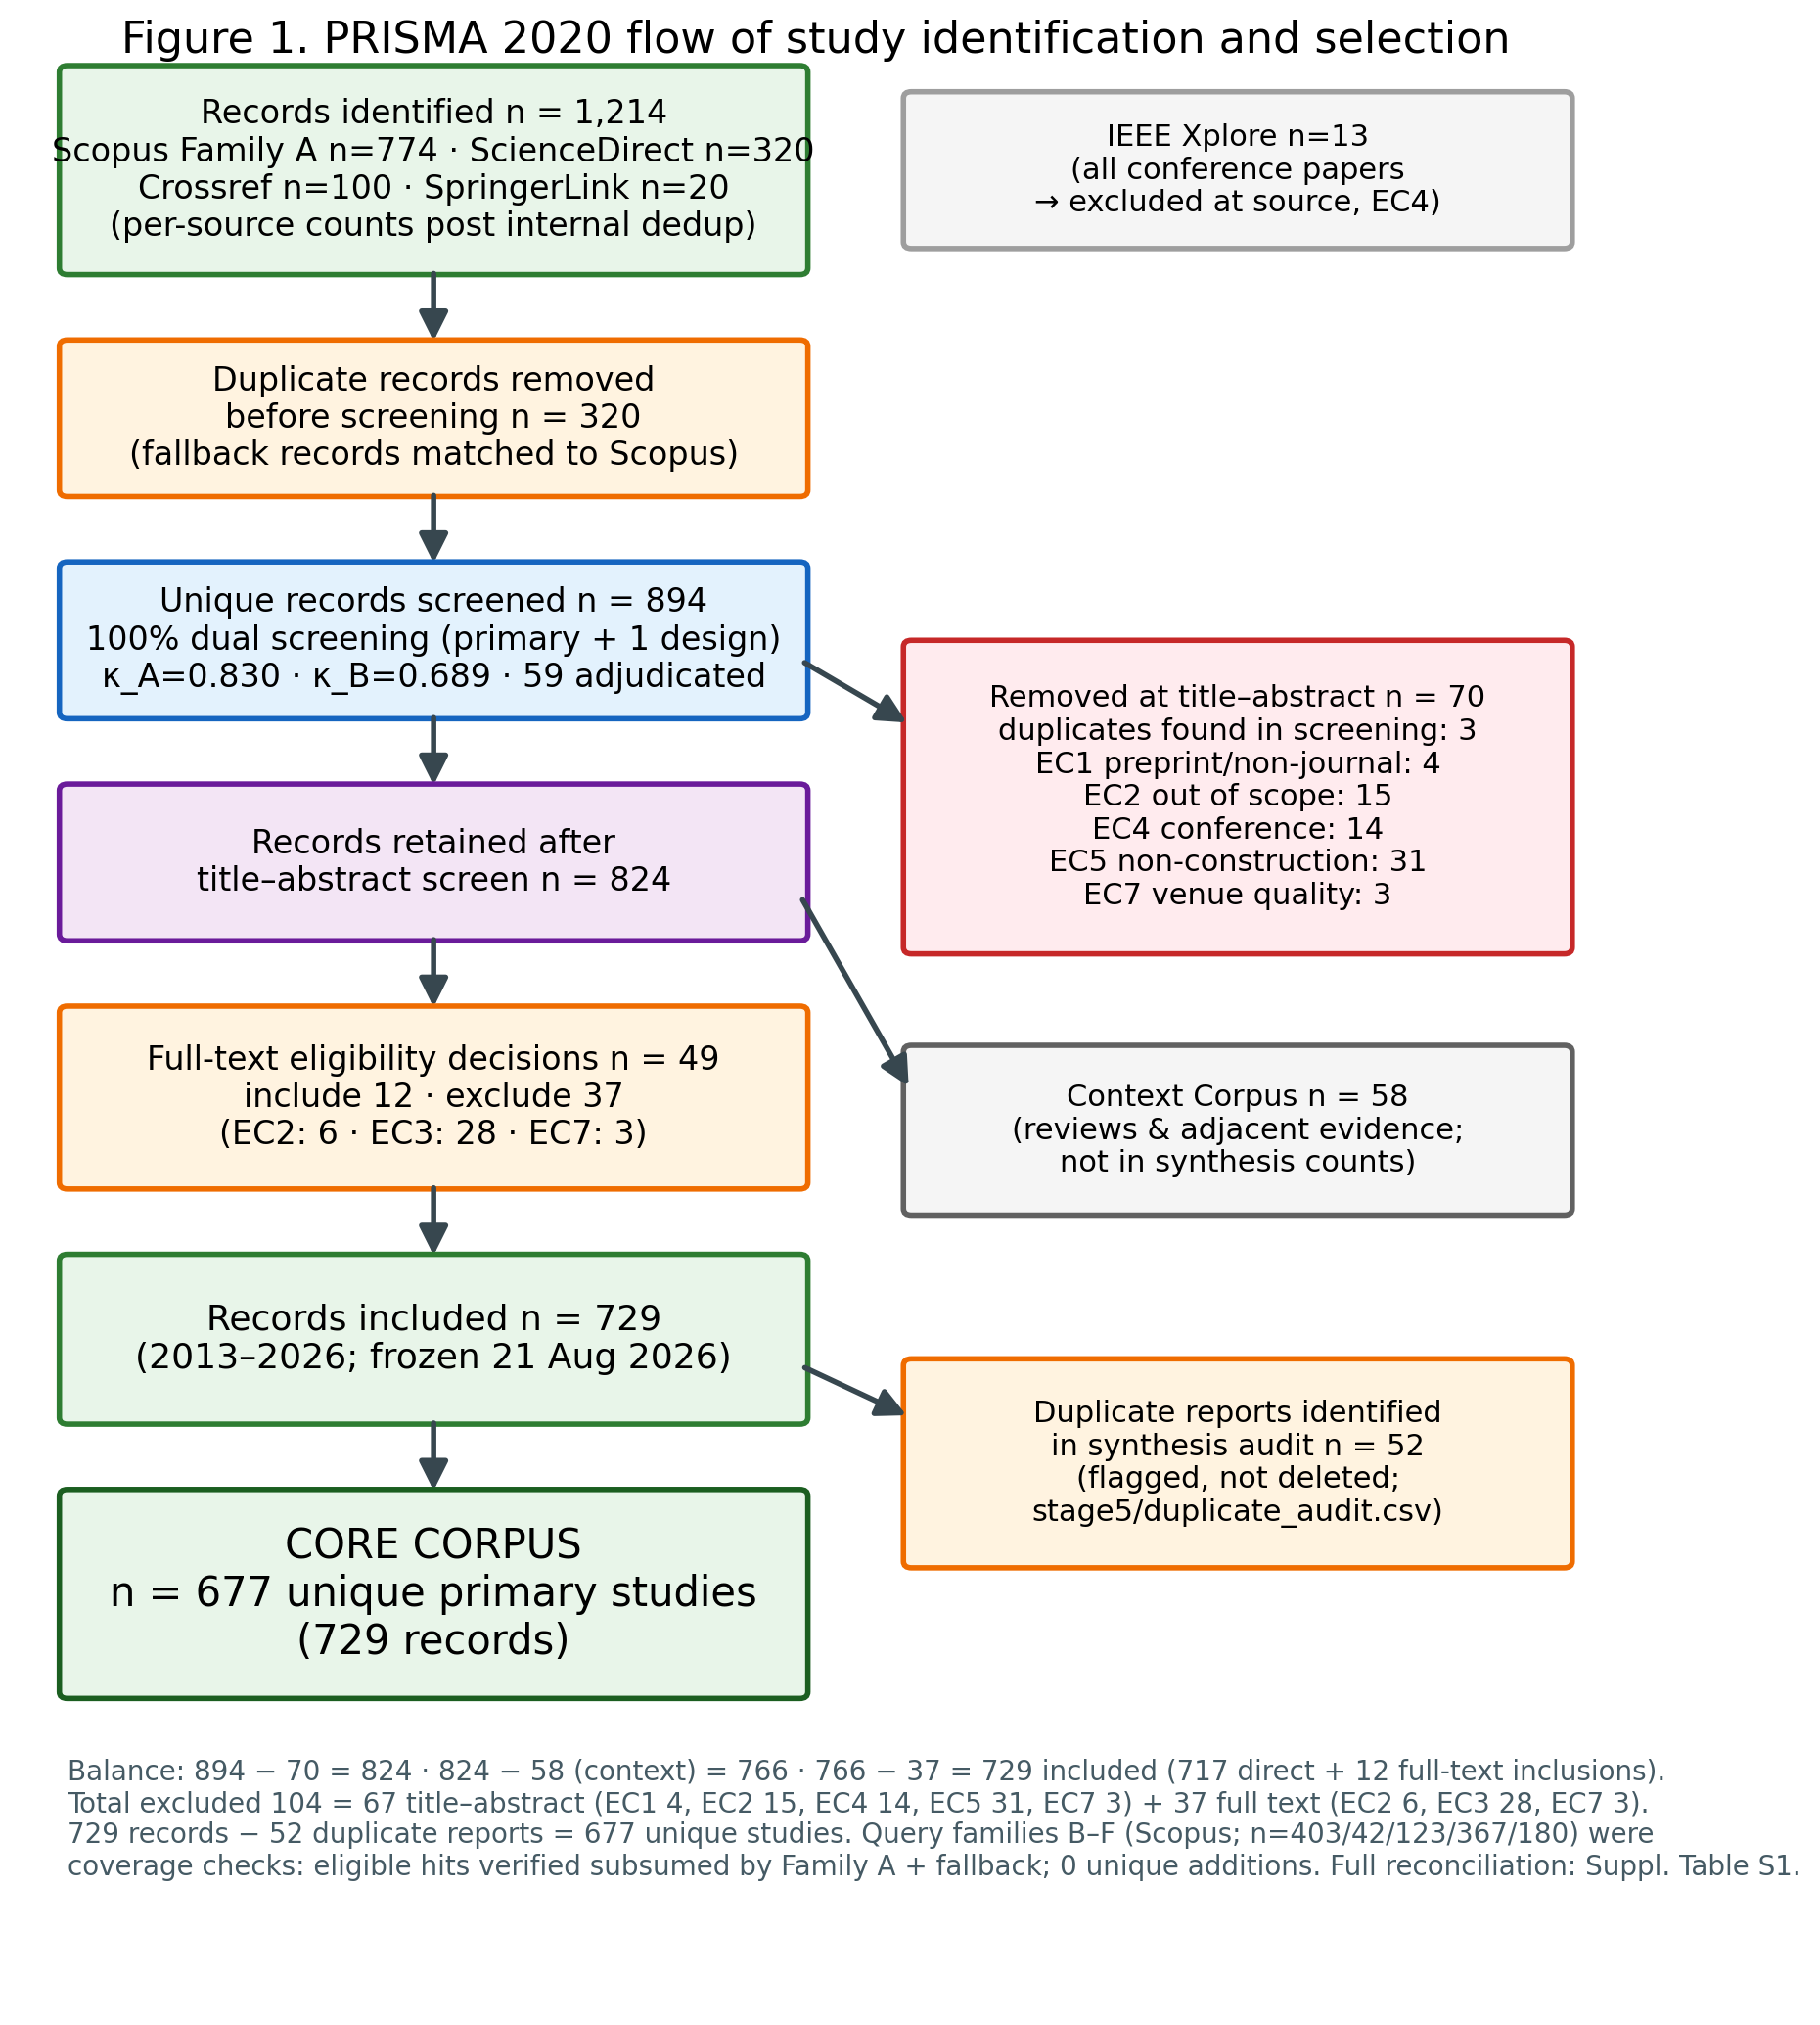
\includegraphics[width=0.95\textwidth]{Fig1.png}
\caption{PRISMA 2020 flow of study identification and selection. The flow balances at every step: 894 $-$ 70 (title--abstract removals, incl. 3 duplicates) = 824; $-$ 58 (Context Corpus) = 766; $-$ 37 (full-text exclusions) = 729 included records = 677 unique studies + 52 duplicate reports flagged in synthesis. EC tallies aggregate both stages (total 104); families B--F contributed no unique records (coverage checks). Full reconciliation: Supplementary Table S1}\label{fig1}
\end{figure}

\section{Low-Carbon Geopolymers as Clean and Circular Technology}

This section equips the general clean-technology reader with the material facts the rest of the review presumes; specialists may proceed to Section 4.

Geopolymers and alkali-activated materials are binders formed when aluminosilicate-rich precursors dissolve and repolymerize in alkaline media, producing three-dimensional gel networks --- sodium-aluminosilicate-hydrate (N-A-S-H) in low-calcium systems, calcium-(sodium)-aluminosilicate-hydrate (C-(N-)A-S-H) where slag-derived calcium participates --- that bind aggregates much as Portland cement hydrates do. Two facts give the family its clean-technology significance. First, the carbon arithmetic: Portland clinker emits most of its CO$_2$ from limestone calcination and kiln fuel, whereas AAM precursors are predominantly industrial residues requiring no calcination, so cradle-to-gate reductions of 40--80\% relative to comparable Portland concretes are repeatedly reported, with the alkaline activator --- particularly sodium silicate --- dominating the remaining footprint. Second, the circularity arithmetic: the principal precursors are wastes with disposal liabilities of their own --- pulverized fuel ash from coal combustion, ground granulated blast-furnace slag from ironmaking, and more challenging streams such as red mud from alumina refining, mine tailings, and biomass ashes --- so every tonne bound into a performing material is subtracted from an impoundment or landfill.

The same facts define the difficulty. Performance depends on a web of coupled variables: precursor mineralogy and amorphous (reactive) content; oxide chemistry, conventionally tracked through SiO$_2$/Al$_2$O$_3$, CaO/SiO$_2$, and Na$_2$O/Al$_2$O$_3$ ratios; activator type, modulus, and dosage; liquid-to-binder ratio; and curing temperature and duration, which govern early reaction kinetics especially for low-calcium systems. Unlike clinker, whose global uniformity was engineered over a century, waste-derived precursors vary between sources, between plants, and between batches --- the central reason a universal prescriptive mix design has never emerged, and one of two structural motivations for data-driven methods. The other is verification tempo: strength qualification conventionally waits 28 days, so purely empirical optimization is slow precisely where the design space is widest. Two further developments frame the AI literature this review audits. One-part ("just add water") formulations, in which solid activators are dry-blended with precursors, trade some performance flexibility for logistics and safety advantages that matter at scale --- and, as Section 20 argues, for automation friendliness. And durability questions --- carbonation behavior of lower-calcium gels, chloride transport, sulfate and acid response, freeze--thaw performance --- remain the family's key technical debate, which is why durability targets are a growing minority of the modeling corpus (16.5\% of studies) and why service-life prediction recurs throughout Sections 8--15.

Deployment context completes the picture. AAMs are not exotic: precast elements, pavements, and niche structural applications exist on several continents, and standards activity is under way in multiple jurisdictions. Yet acceptance frameworks remain calibrated to Portland chemistry, feedstock supply is being reshaped by decarbonization itself --- coal-plant retirements and hydrogen ironmaking will shrink and alter fly ash and slag streams, pushing the field toward the more variable residues where data-driven methods are most needed --- and environmental claims made mix-by-mix require the life-cycle discipline that Section 11 finds largely absent. The clean-technology promise of geopolymers, in short, is real, conditional, and quantitative --- exactly the kind of promise whose realization can be audited, which is what the remainder of this review does.

\section{Evolution of the Field and Position Among Prior Reviews}

The corpus's growth curve is the first empirical result (unique studies throughout, n = 677). From isolated antecedents (2013--2015, six studies) the literature idles below fifteen papers annually until 2020, doubles through 2021--2022 (38, then 62), plateaus briefly in 2023 (60), and then detonates: 130 studies in 2024, 178 in 2025, and 172 in 2026 --- the last figure not like-for-like, since four months of 2026 were unindexed at freeze (it includes one in-press item indexed 2027). Seventy-one percent [95\% CI 67.4--74.2] of everything this review analyzes was published since January 2024 --- the final 32 months of its fourteen-year window. Any synthesis of this field is therefore a synthesis of its most recent third --- and any review frozen earlier missed most of the phenomenon. The venue distribution tells a second story: the literature publishes overwhelmingly in construction-materials journals (Construction and Building Materials leads with 57 studies; Journal of Building Engineering, Case Studies in Construction Materials, and Materials follow), with rapid-turnaround venues (Asian Journal of Civil Engineering, 35; Scientific Reports, 32) absorbing much of the post-2024 surge, and cleaner-production venues (Journal of Cleaner Production, 13) hosting the environmentally coupled minority. Computing venues are essentially absent --- a fact confirmed independently by the IEEE Xplore search (Section 2), and one that explains the methodological porting failures documented in Section 15: the field imports algorithms from machine learning but not the evaluation culture that accompanies them.

Prior reviews map onto this landscape as valuable but differently scoped instruments. Landscape surveys --- most systematically a PRISMA review of 184 studies to December 2023 \citep{nguyen2025} --- characterize forms, precursors, algorithms, and dataset sizes, and correctly flag data scarcity; property-focused reviews synthesize compressive-strength prediction for fly-ash systems \citep{rathnayaka2024}, broader systematic surveys span geopolymer and adjacent eco-concretes \citep{ali2024,alaneme2023}; and a recent narrative review advances a "dual-driven" data-plus-mechanism framing and knowledge-graph outlook that anticipates one strand of Section 9 \citep{zheng2025}. This review differs from all of them on four axes at once. Temporally, its corpus (677 unique studies, through August 2026) is 3.7 times the largest predecessor and covers the surge years that reshaped the field. Analytically, it audits rather than catalogues: prior reviews report what studies claim; Sections 8--15 grade claims against practice. Thematically, it treats trustworthiness, environmental quantification, and deployment as first-class dimensions, none of which any predecessor systematically assesses. And instrumentally, it releases its coded corpus and audit tables as reusable infrastructure. Table 1 details the comparison; the short version is that predecessors asked "what has been done?", while this review asks "what has been established, and what would it take to deploy it?" --- the question a clean-technology venue requires.

\begin{table}[htbp]
\caption{Prior reviews at the AI $\times$ geopolymer intersection versus this review}
\centering
{\footnotesize
\begin{tabular}{p{0.068\textwidth}p{0.144\textwidth}p{0.180\textwidth}p{0.088\textwidth}p{0.132\textwidth}p{0.136\textwidth}p{0.064\textwidth}p{0.108\textwidth}}
\toprule
Review & Year/venue & Corpus \& window & Trust audit & Physics audit & LCA/env audit & Deployment & PRISMA \\
\midrule
Nguyen et al. & 2025, Materials Today Sustainability & 184 studies, to Dec 2023 & partial (data quality) & no & no & no & yes \\
Zheng et al. & 2025, J. Building Engineering & narrative & interpretability only & dual-driven framing & no & no & no \\
Rathnayaka et al. & 2024, Constr. Build. Mater. & FA-GPC strength only & no & no & no & no & partial \\
Ali et al. & 2024, Constr. Build. Mater. & multi-concrete SLR & no & no & no & no & yes \\
Alaneme et al. & 2023, SN Applied Sciences & GPC production & no & no & no & no & no \\
THIS REVIEW & 2026 & 677 unique studies (729 records), to Aug 2026 & 8-dim scorecard & 5-level claimed-vs-verified audit & evidentiary ladder incl. ISO check & D-axis + roadmap & yes + primary+1 dual screen \\
\bottomrule
\end{tabular}}
\end{table}

\section{A Multidimensional Taxonomy for AI-Enabled Geopolymer Research}

\subsection{Why existing organizations fail}

Prior reviews organize this literature by algorithm family or by predicted property. Both organizations collapse under the corpus assembled here. An algorithm-centric scheme reduces to a catalogue of ensembles and neural networks that says nothing about whether a study can be trusted, transferred, or translated; a property-centric scheme places three-fifths of the field in a single compressive-strength bin. More fundamentally, the questions this review asks --- how trustworthy, how physically grounded, how environmentally quantified, how close to deployment --- are orthogonal to both. No single hierarchy can carry them, because they are independent dimensions of the same study: a paper may couple carbon into a genetic optimization while reporting no uncertainty, or embed reaction physics while never leaving its training envelope.

Three candidate taxonomies were therefore developed and scored against six criteria (novelty, scientific value, interpretability, coding stability, journal relevance, and downstream usefulness; Supplementary Table S4): a single-axis AI-maturity ladder, a six-axis faceted classification, and a seven-stage clean-technology translation pipeline. The faceted classification scored highest (52/60) and was adopted as the analytical instrument; the other two are retained deliberately as \emph{views} of it, as explained below.

\subsection{The six axes}

Every Core Corpus study receives a six-part profile rather than a single bin:

\textbf{M --- Material system.} Fly ash, slag, and their blends; metakaolin and calcined clays; red mud; mine tailings; biomass ashes; recycled-aggregate and multi-waste systems; one-part formulations; geopolymer-stabilized soils and backfills.

\textbf{T --- AI task.} Property prediction; classification; microstructure and image analysis; single- and multi-objective optimization; inverse design and recommendation; uncertainty-focused prediction; experiment selection (active/sequential learning); autonomous experimentation.

\textbf{R --- Trust profile.} Eight binary-with-partial flags mirroring the scorecard: explainability, uncertainty quantification, calibration, robustness, out-of-distribution evaluation, external validation, physical consistency, reproducibility. A SHAP plot alone earns a partial explainability credit; a chemically interrogated explanation earns full credit.

\textbf{P --- Physics integration.} Type I, purely data-driven; Type II, domain quantities (oxide ratios, moduli) included as ordinary features; Type III, domain knowledge shaping model structure or feature construction (knowledge graphs, chemistry-guided architectures); Type IV, physics- or chemistry-constrained learning (embedded governing equations, PINN losses); Type V, hybrid mechanistic--ML models (thermodynamic simulation coupled to learning). Assignment is conservative: ambiguity resolves downward, and claimed labels are audited rather than accepted (Section 9).

\textbf{E --- Environmental function.} None explicit; waste valorization; durability and service life; cost; carbon quantification; CO$_2$ uptake; life-cycle assessment, itself graded none / emission factors / partial LCA / ISO-boundary LCA (Section 11).

\textbf{D --- Deployment maturity.} Laboratory prediction $\rightarrow$ externally validated model $\rightarrow$ formulation recommendation $\rightarrow$ process optimization $\rightarrow$ pilot implementation $\rightarrow$ digital-twin integration $\rightarrow$ adaptive experimentation $\rightarrow$ semi-autonomous $\rightarrow$ autonomous discovery, with adaptive stages sub-coded \emph{simulated} versus \emph{physical} --- a distinction the pilot extraction proved essential, since every adaptive study identified operates retrospectively on literature data.

Coding rules were fixed before extraction: multi-label T with a single primary label under a fixed priority order (task percentages in this review use primary labels and therefore sum to 100\%); multi-label M, whose material-system shares intentionally sum to more than 100\% because blended systems carry every applicable label; environmental credits require quantification, so the word "sustainable" earns nothing; trust flags require demonstrated evidence. All 729 record profiles, with the 52 duplicate reports flagged, are released in the research artifact.

\subsection{One coding, three views}

The two rejected taxonomies survive as projections of the six-axis coding, and this construction is itself methodological: it removes the arbitrariness that reviewers rightly suspect in bespoke classification schemes. Projecting each study's task and deployment codes onto an ordered capability scale yields the \textbf{AI-maturity ladder} --- statistical modeling, ML prediction, explainable AI, uncertainty-aware AI, physics-informed AI, inverse design, adaptive experimentation, autonomous discovery --- whose population over time is this review's single most consequential figure (Figure 2): the lower rungs crowd with hundreds of studies while the top two rungs hold, respectively, three simulated demonstrations and none at all. Projecting task and environmental codes onto functional stages yields the \textbf{clean-technology translation pipeline} --- understand, predict, trust, design, green-assess, adapt, discover --- which orders the synthesis that follows (Sections 7--14). Because ladder, pipeline, and facets are all views of one pre-registered coding, any disagreement about a study's placement is resolvable by inspecting its released profile rather than by argument.

\subsection{What the taxonomy immediately reveals}

Even before detailed synthesis, the joint distributions expose the field's shape. Task and trust axes are nearly independent in the worst way: the 95.7\% of studies performing prediction or optimization carry no more trust practice than the corpus average, and 60.1\% of all studies exhibit no detectable trust practice whatsoever. The physics axis is bimodal, and its split partitions by claim status: a mass at Types I--II (96.0\% of the corpus by demonstrated content) and, at Types III--V, twenty-seven \emph{claimed} profiles (4.0\%) of which nine survive verification (1.3\%; Section 9's audit). Partitioned by demonstrated content instead, 98.1\% of the corpus operates at Type II or below --- the stronger statement of the same fact. The environmental axis contradicts the field's self-presentation: nearly half of a literature framed around sustainability quantifies no environmental variable (Section 11). And the deployment axis terminates, across all 677 studies, at decision-support tools: no pilot implementation, certification engagement, or physical discovery loop was detected in the coded corpus. These four asymmetries --- trust, physics, environment, deployment --- define the gap structure (Section 19) and the roadmap (Section 20) of this review.

\begin{figure}[htbp]
\centering
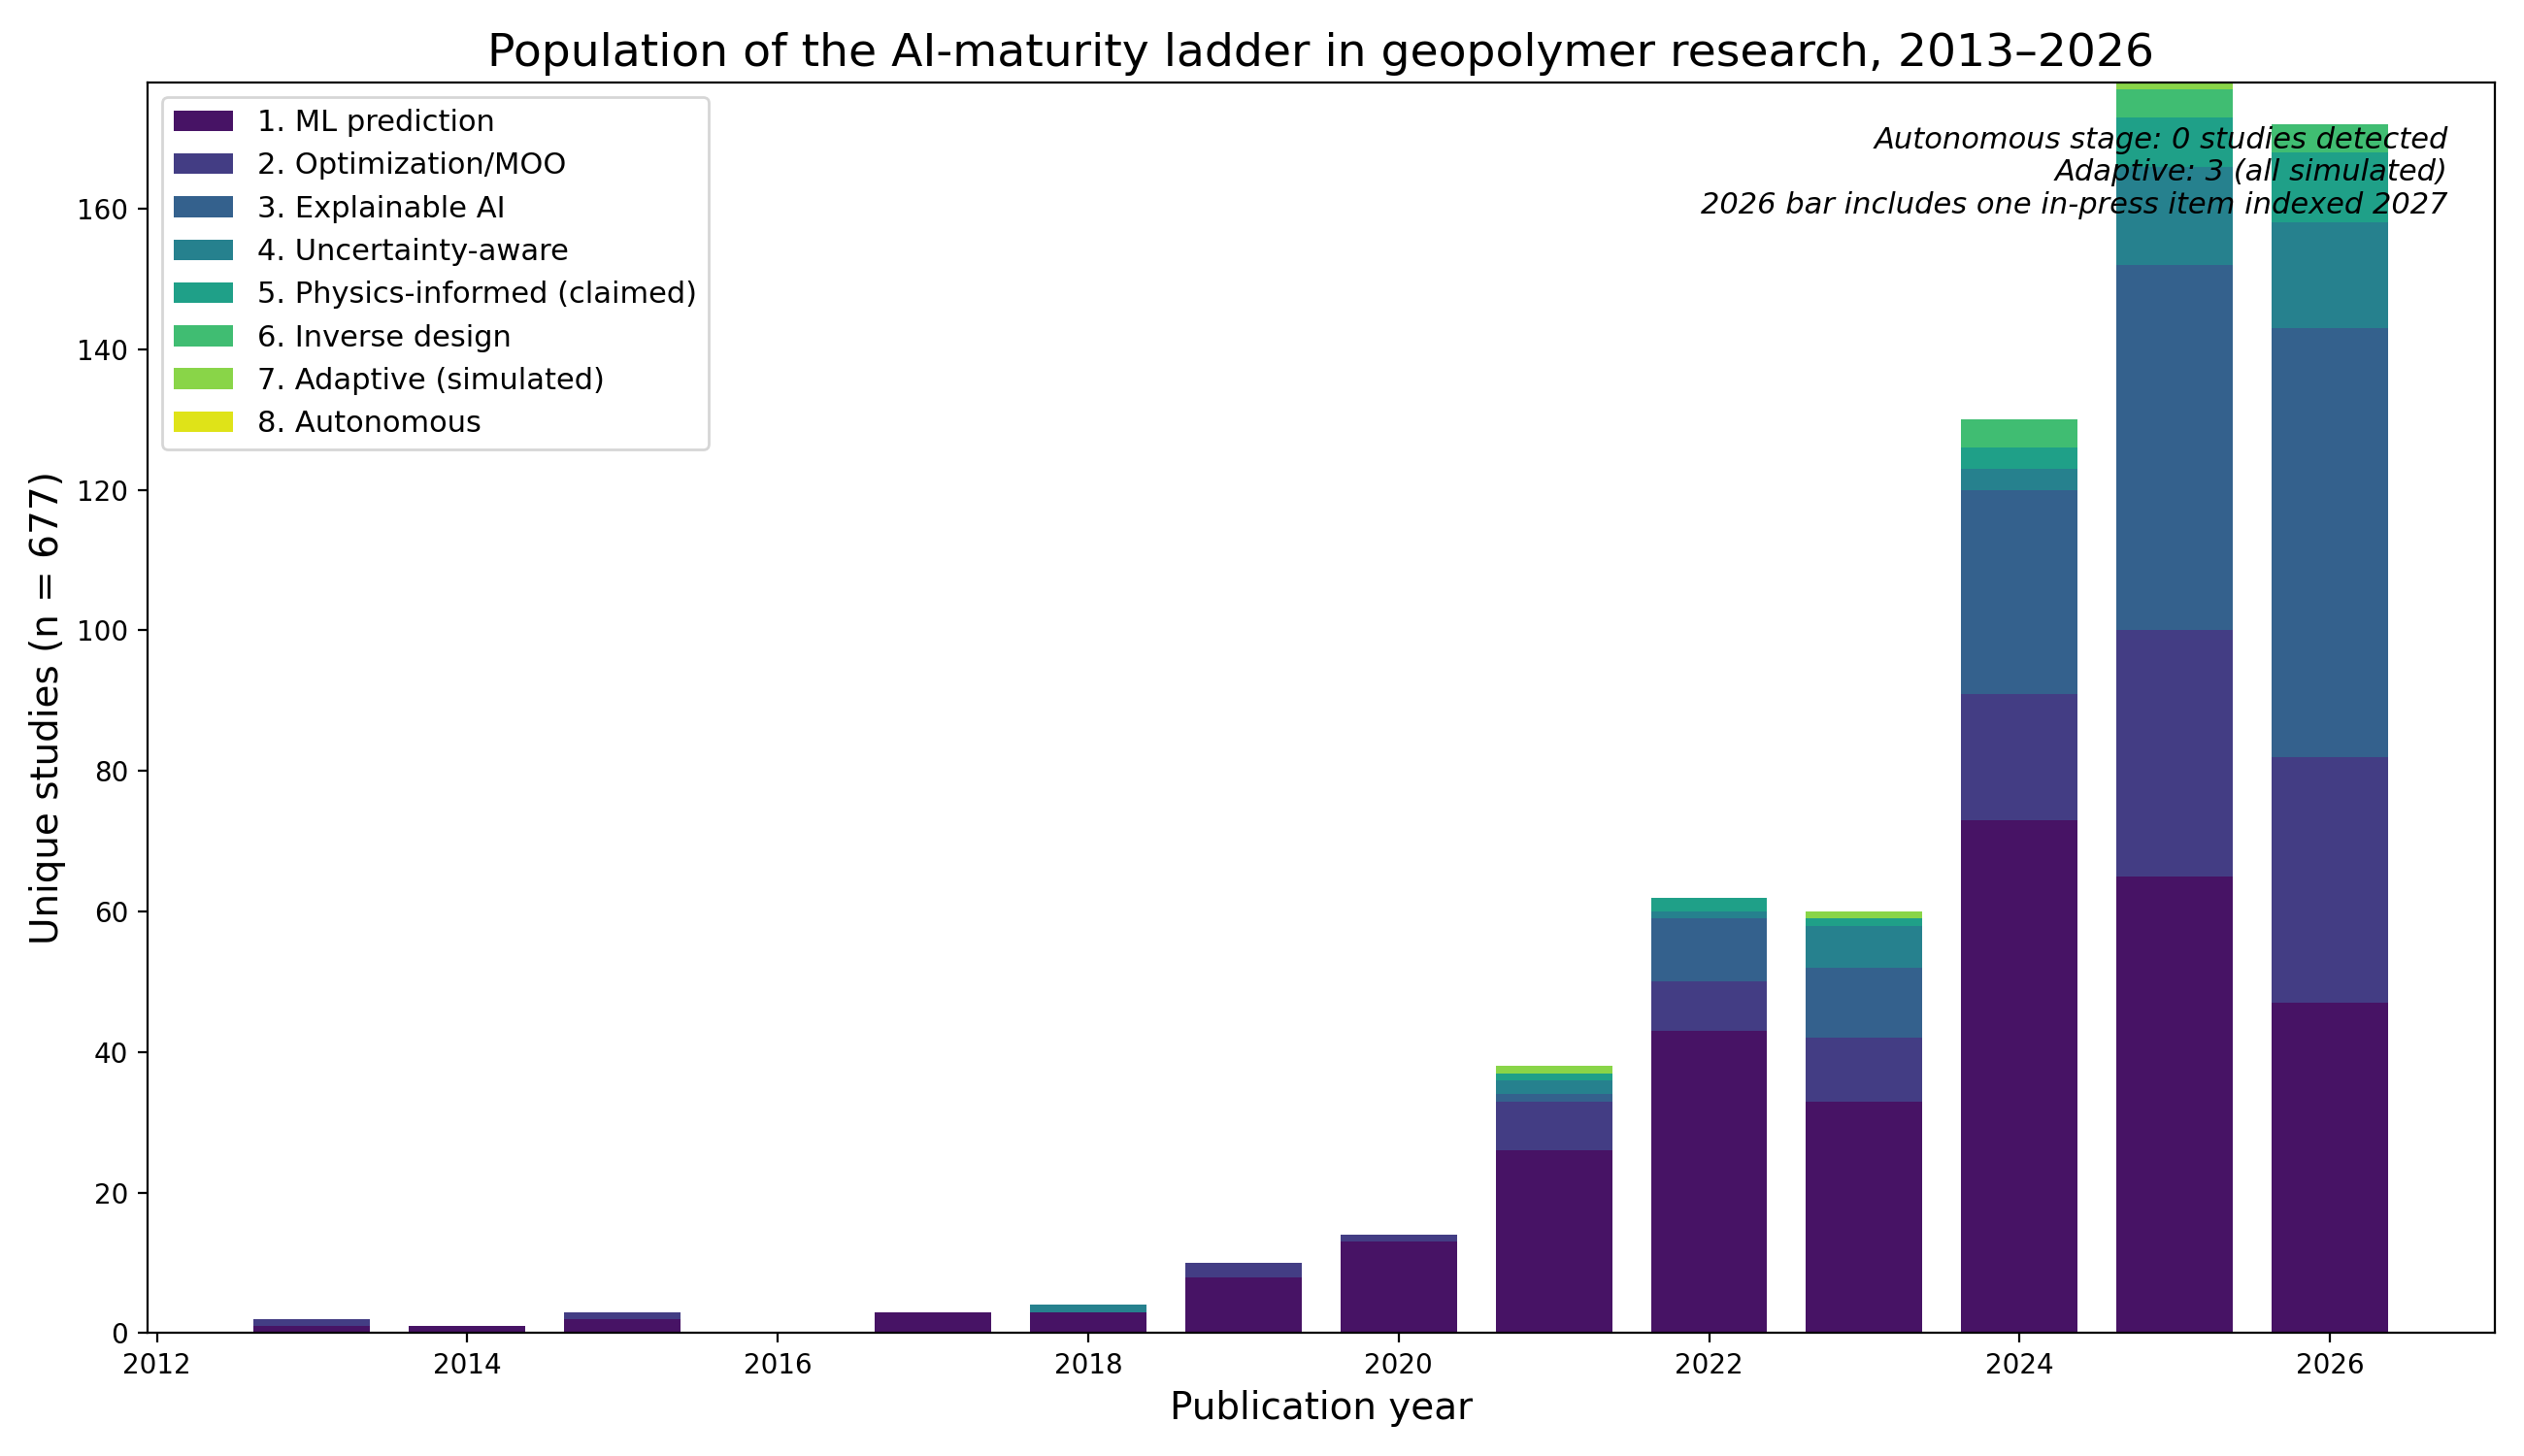
\includegraphics[width=0.95\textwidth]{Fig2.png}
\caption{Population of the AI-maturity ladder in geopolymer research, 2013--2026 (view A of the taxonomy; unique studies, n = 677). "Physics-informed" counts claimed labels --- Fig. 5 reports the claimed-versus-verified audit. The 2026 bar includes one in-press item indexed 2027 and is not like-for-like (four months unindexed at freeze)}\label{fig2}
\end{figure}

\begin{figure}[htbp]
\centering
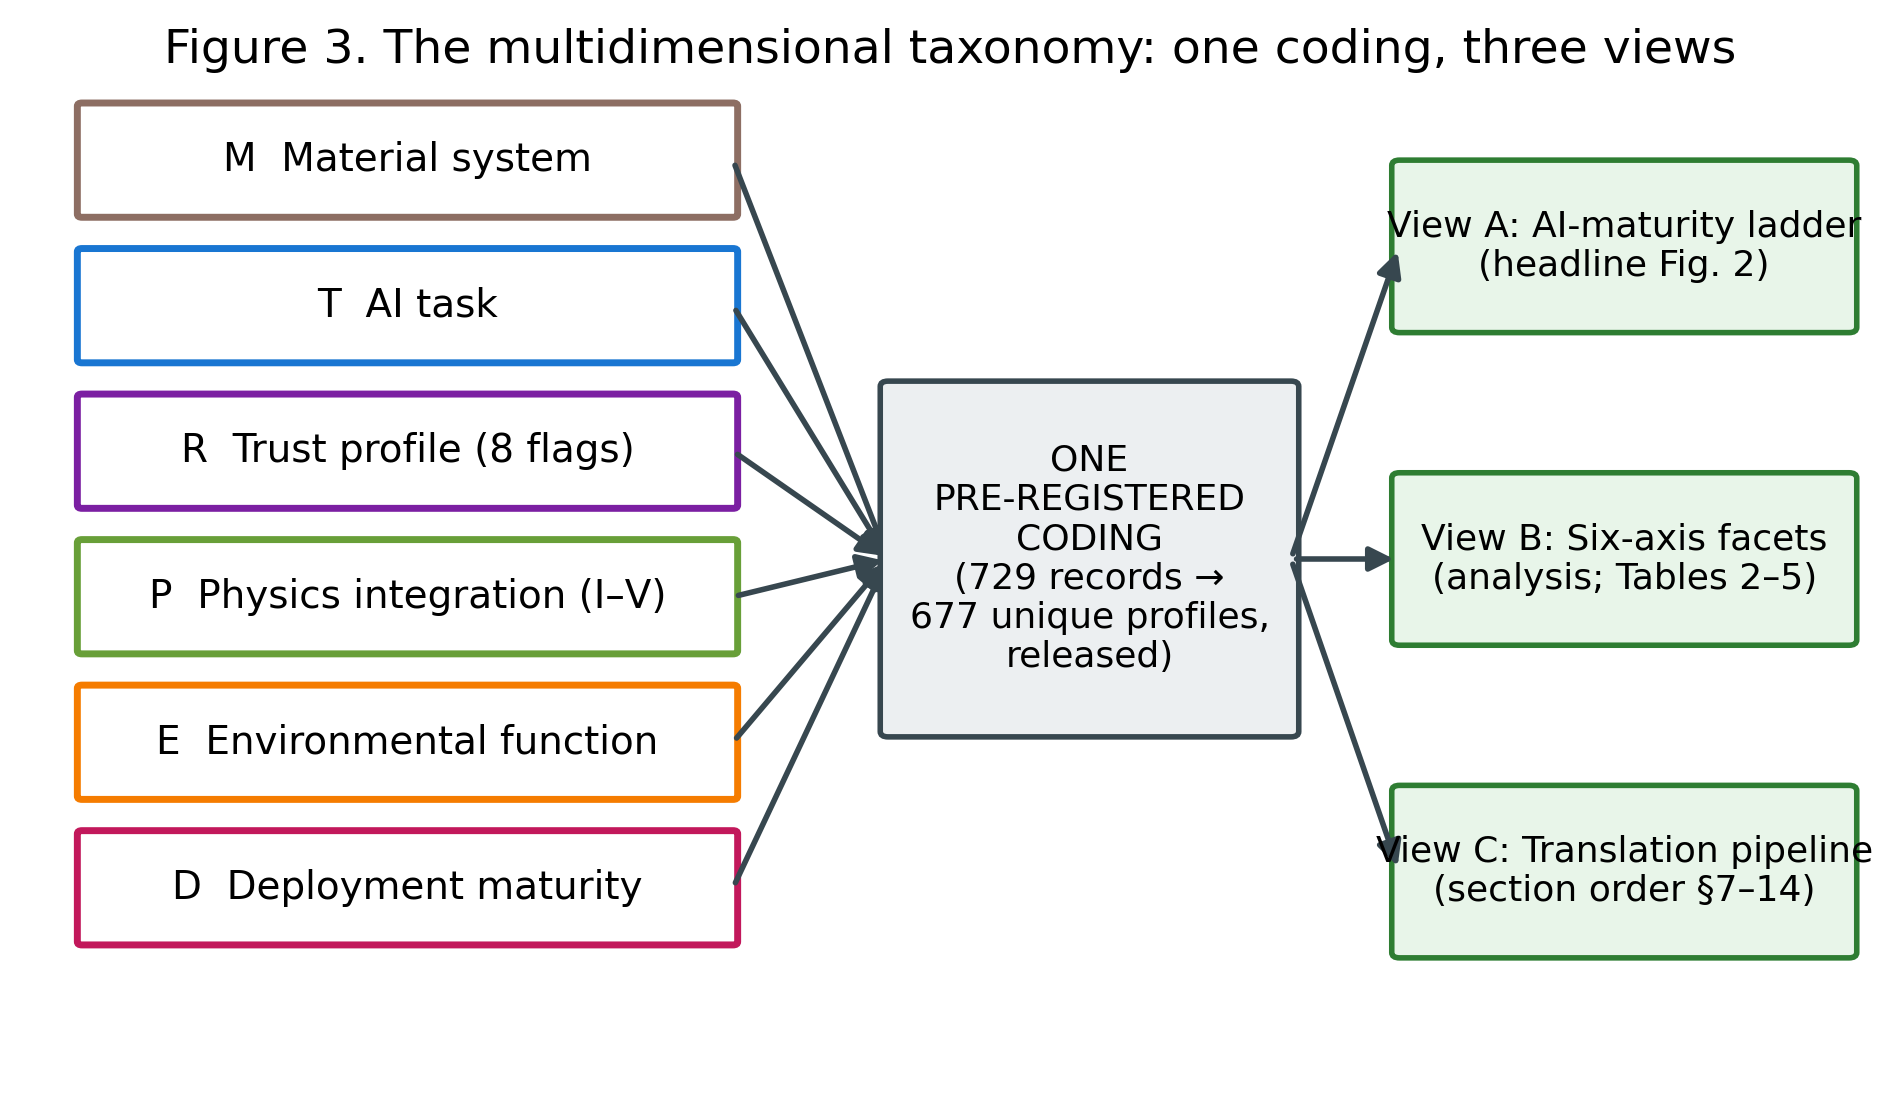
\includegraphics[width=0.95\textwidth]{Fig3.png}
\caption{The multidimensional taxonomy: one pre-registered coding, three views}\label{fig3}
\end{figure}

\begin{table}[htbp]
\caption{Material system $\times$ primary AI task (unique studies, n = 677; material axis is multi-label, so totals exceed 677; the Opt column includes metaheuristically tuned predictors --- Table S9)}
\centering
{\footnotesize
\begin{tabular}{p{0.286\textwidth}lllllllll}
\toprule
Material & Pred & Opt & MOO & Inv & Class & Micro & P+UQ & Adapt & Total \\
\midrule
fly-ash & 95 & 50 & 8 & 2 & 0 & 4 & 0 & 0 & 159 \\
FA-slag & 89 & 46 & 10 & 4 & 3 & 1 & 1 & 1 & 155 \\
slag & 62 & 27 & 4 & 1 & 4 & 3 & 0 & 0 & 101 \\
metakaolin/clay & 24 & 12 & 2 & 0 & 0 & 1 & 0 & 0 & 39 \\
red-mud & 6 & 1 & 0 & 0 & 0 & 0 & 0 & 0 & 7 \\
tailings & 4 & 3 & 0 & 1 & 0 & 0 & 0 & 0 & 8 \\
biomass-ash & 25 & 6 & 0 & 0 & 0 & 2 & 0 & 0 & 33 \\
recycled-aggregate & 18 & 4 & 2 & 2 & 0 & 2 & 0 & 0 & 28 \\
one-part & 12 & 6 & 0 & 1 & 0 & 0 & 0 & 0 & 19 \\
stabilized-soil & 31 & 13 & 1 & 2 & 0 & 1 & 0 & 0 & 48 \\
mixed/other-AAM & 124 & 44 & 10 & 3 & 4 & 5 & 2 & 2 & 194 \\
\bottomrule
\end{tabular}}
\end{table}

\section{Materials, Data, and Representation: What the Models Actually See}

\textbf{Material coverage mirrors industrial availability, not future need.} Coded by material system --- a multi-label axis, so shares intentionally sum to more than 100\% because blended systems carry every applicable label --- the corpus concentrates where data is easiest: fly-ash systems (23.5\% of studies), fly-ash/slag blends (22.9\%), and slag systems (14.9\%) together dominate, with a long tail of blended and miscellaneous AAMs (28.7\%). Geopolymer-stabilized soils form a distinct applied cluster (7.1\%); metakaolin and calcined clays (5.8\%), biomass ashes (4.9\%), and recycled-aggregate systems (4.1\%) are minorities; and the streams whose valorization is hardest and environmentally most valuable are the least modeled --- one-part systems 2.8\%, mine tailings 1.2\%, red mud 1.0\%. The asymmetry matters prospectively: the fly ash and slag on which the models train are precisely the feedstocks that decarbonization will shrink (Section 3), while the variable residues that will replace them are nearly absent from the training distributions --- an anticipatable domain shift the field is not preparing for (G2).

\textbf{Representation is compositional, shallow, and lossy.} The canonical input vector concatenates mix proportions, activator parameters (molarity, modulus, activator-to-binder ratio), curing temperature and age, and --- in the better half of the corpus --- precursor oxide fractions or derived ratios. What it omits is what a chemist would ask first: amorphous versus crystalline content, particle size distribution and fineness, dissolution reactivity, and calorimetric signatures. These omissions are not oversights of individual authors but artifacts of the supply chain: compiled literature data can only carry what source papers reported, and source papers rarely report reactivity. The consequence surfaces throughout the synthesis --- models that cannot distinguish two fly ashes with identical oxide totals but different glass contents will attribute the difference to noise, capping achievable accuracy and corrupting transferability. The corpus's own best counter-examples --- a reactivity-assessment framework for fifteen solid wastes \citep{song2025}, and rapid ML-based reactivity classification for fly-ash recycling \citep{qi2022} --- point to the repair: reactivity descriptors as first-class features, which the benchmark proposal (G6) operationalizes.

\textbf{Dataset practice.} The quantitative anatomy of the field's datasets --- compilation dominance, characteristic sizes in the low hundreds, recirculation of a few standard databases, documented duplicate contamination, and the near-absence of provenance --- is treated as part of the validation audit (Section 15.1), because its consequences are evidentiary rather than material. Here one number suffices to frame it: across 677 studies, no shared benchmark exists, and no two research groups can currently be shown to have evaluated on provably identical data. Every comparative claim in the field should be read in that light.

\section{Prediction-Centric Machine Learning: The Field's Massive, Repetitive Core}

Property prediction and the optimization built atop predictive surrogates together constitute 95.7\% [93.9--97.0] of the corpus (the remainder: classification 1.6\%, microstructure and image analysis 2.2\%, adaptive experiment selection 0.4\%). The split within that figure --- 61.7\% coded prediction, 34.0\% optimization and inverse design --- is criterion-sensitive and should be read as indicative: both independent reliability recodes (human and procedural; Table S9) show the optimization label absorbing metaheuristically \emph{tuned} predictors alongside genuine design-space search, so the prediction-type share is in truth higher and demonstrated design search lower (roughly 10--17\%; the strictly-labelled multi-objective and inverse-design work, 6.8\%, is its floor). This section characterizes the core by its patterns; per the invalid-comparison rule, it ranks no models.

\textbf{Target monoculture.} Compressive strength --- usually at 28 days, often alone --- is the overwhelming target, with fresh properties (slump, setting, rheology), other mechanical properties (tensile, flexural, elastic modulus), and durability indicators (carbonation depth, chloride ingress, freeze--thaw loss, acid/sulfate response) forming successively smaller shells. Durability targets are the scientifically valuable growth area (17.0\% of studies touch them), because they are where AAMs' open technical questions live and where measurement cost makes surrogate models genuinely useful; the durability cluster also hosts a disproportionate share of the corpus's methodological best practice (Sections 8--9).

\textbf{Algorithmic convergence.} The field has converged on gradient-boosted tree ensembles and feed-forward networks as workhorses, wrapped --- in a distinctly regional publication style --- with metaheuristic tuners of every taxonomic family (genetic, swarm, bat, grey-wolf, firefly and successors). Within-study controlled comparisons repeatedly show competent ensembles clustering within small margins of each other; the proliferation of hybrid-optimizer variants adds tuning convenience more often than demonstrated generalization benefit, and no variant's superiority survives transport across datasets (Section 18). The methodological energy spent on optimizer novelty contrasts sharply with the near-zero investment in calibration and validity assessment that Sections 8 and 15 document --- a misallocation this review regards as the core cluster's defining feature.

\textbf{The workflow is standardized; its evaluation is not.} A canonical pipeline --- compile literature data, engineer features, split randomly, tune by cross-validation, report R$^2$/RMSE/MAE, close with a SHAP plot --- now constitutes a template so stable that dozens of papers differ only in dataset and optimizer. Standardization is not itself a defect; the defect is that the template froze \emph{before} the evaluation practices that make predictions decision-grade (group-aware splits, external tests, coverage reporting) entered it. The template's very stability, however, is also the opportunity: because the field repeats one workflow, upgrading that workflow --- the immediate roadmap tier (I2--I3) --- upgrades hundreds of future studies at once.

\textbf{What prediction has genuinely bought.} Read charitably, the core cluster has established three durable facts: that compositional and curing variables suffice to predict 28-day strength within a few MPa \emph{inside} well-sampled envelopes; that curing temperature, activator chemistry, and calcium availability dominate those envelopes' response surfaces; and that surrogate accuracy is no longer the binding constraint on AI-assisted geopolymer development. Everything the field now lacks lies beyond accuracy --- which is why the sections that follow, rather than this one, carry the review's weight.

\section{Explainable and Trustworthy AI: Interpretation Without Reliability}

\subsection{The scorecard and what it measures}

Trustworthiness was assessed per study on eight dimensions, each answering an operational question (Table 3): explainability (why did the model predict this?), uncertainty quantification (how confident is it?), calibration (is that confidence meaningful?), robustness (is performance stable under perturbation?), out-of-distribution behavior (does it survive unseen chemistry?), external validation (was genuinely independent data used?), physical consistency (are outputs chemically plausible?), and reproducibility (could another group repeat this?). These dimensions are deliberately not aggregated into a single score: a study strong in interpretation and absent in validation is a different object from its converse, and the field's pattern turns out to be precisely such an asymmetry.

\subsection{The asymmetry: explainability boomed, reliability did not}

Across the 677-study corpus, 60.1\% [95\% CI 56.4--63.7] of studies exhibit no detectable trust practice on any dimension. The exception is explainability, present in 29.1\% [25.8--32.6] of studies and growing steeply after 2023 --- overwhelmingly as SHAP attribution, with partial-dependence analysis and permutation importance as minor variants; the reliability recode marks this as the scorecard's most liberally awarded flag (Table S9), so if anything the asymmetry documented here is understated. The remaining dimensions stagnate at levels an order of magnitude lower: uncertainty quantification 6.2\% [4.6--8.3], out-of-distribution or transfer evaluation 8.6\% [6.7--10.9], external validation 4.0\% [2.8--5.7], calibration 1.3\% [0.7--2.5], and explicit reproducibility signals --- a resolvable code or data repository --- near 1\% (all detected at title--abstract--keyword level; Section 21 quantifies the resulting under-detection bound). Interpreted through the scorecard, the field has adopted the \emph{cheapest} trust dimension, the one installable in three lines of code atop any gradient-boosting model, while leaving the expensive dimensions --- those requiring new data, new experiments, or statistical discipline --- essentially untouched. Explainability without reliability is a hazardous combination: SHAP values computed on an uncalibrated, unvalidated model explain a function whose relationship to reality is unknown, and chemically plausible-looking attributions can lend unearned credibility to predictions that would fail outside the training envelope (Section 15).

A second-order concern compounds this. Because roughly nine in ten SHAP analyses in the corpus run on models trained from the same few compiled literature databases (Section 6), their "insights" --- curing temperature matters, molarity matters, calcium content matters --- are less independent discoveries than repeated re-descriptions of one data distribution. The corpus contains dozens of near-identical importance rankings presented as findings; their convergence is evidence about the shared dataset, not cumulative evidence about geopolymer chemistry.

\subsection{The calibration frontier: demonstrated, cheap, and ignored}

The corpus's nine calibration-evaluating studies (1.3\%) demonstrate that the barrier is cultural, not technical. The strongest practice cluster applies conformal prediction --- distribution-free intervals with finite-sample coverage guarantees --- to standard geopolymer datasets. One exemplar evaluates native and conformalized intervals from uncertainty-capable learners across thirty independent splits with group-leakage control, reporting 90\% nominal coverage empirically honored at 89.6\% \citep{parakhiya2026}; a companion study couples K-fold residual conformal prediction to gradient boosting, achieving interval coverage of 97.0\% at the 90\% level with mean interval width near 1.2 MPa, and pairs it with an applicability-domain analysis discussed below \citep{jagad2026}. A third, methodologically distinct exemplar reaches calibration through Bayesian machinery: an amortized Gaussian-process framework whose prediction-interval coverage tracks nominal levels across the 50--99\% range and whose uncertainty decomposes into epistemic and aleatoric components --- the epistemic share ($\sim$86\%) itself a finding, indicating that better data, not better noise models, is the binding constraint \citep{chan2026}. Notably, these exemplars trace to overlapping author groups: calibrated uncertainty in geopolymer AI is currently a practice of one or two teams, not a diffusing norm. Nothing in these methods is geopolymer-specific or computationally demanding; conformal calibration could be retrofitted to the majority of published pipelines at negligible cost, which is why it heads this review's immediate roadmap priorities (Section 20, I2).

\subsection{Validation: the missing ladder}

External validation --- evaluation on data the modeling process never touched --- appears in 4.0\% [2.8--5.7] of abstracts, and deep extraction suggests even this overstates independent testing: most claimed validation is a held-out split of the same compiled database. Genuinely independent designs are rare enough to enumerate. One decision-support system reports five-fold cross-validation error (MAE 6.23 MPa) alongside an independent-test error (7.86 MPa), the honest degradation between them being exactly the information deployment requires \citep{natarajan2026}; an active-learning study spot-validates its tuned model against newly performed laboratory tests \citep{kazemi2025}; a handful of studies test across precursor sources. No interlaboratory validation and no prospective validation on mixes designed after model training were detected anywhere in the coded corpus --- a finding from the abstract-level screen that was additionally checked by a targeted full-text search of the deep-extraction tier --- and these are the two rungs of the validation ladder that engineering acceptance would actually require (Section 16). The corpus's own most candid assessment of this situation comes from within: the authors of the conformal inverse-design exemplar caution that their high coefficients of determination "mainly reflect dense interpolation within the structured … experimental envelope rather than unrestricted extrapolation" \citep{jagad2026} --- a sentence this review regards as the most important methodological statement in the field, and one that generalizes far beyond its source.

\subsection{Synthesis}

On the trajectory this review evaluates, the trust stage is not failing uniformly; it is failing selectively. Interpretation tools diffused in two years; reliability practices did not diffuse at all. The result is a literature that can increasingly explain its models but still cannot certify them --- and certification, not explanation, is what stands between a strength predictor and a deployable clean-technology instrument. The gap analysis (G1, G2, G7) and roadmap items I2--I3 and E3 (Section 20) address the three missing practices in ascending order of cost: calibration reporting, applicability-domain declaration, and cross-laboratory validation.

\begin{figure}[htbp]
\centering
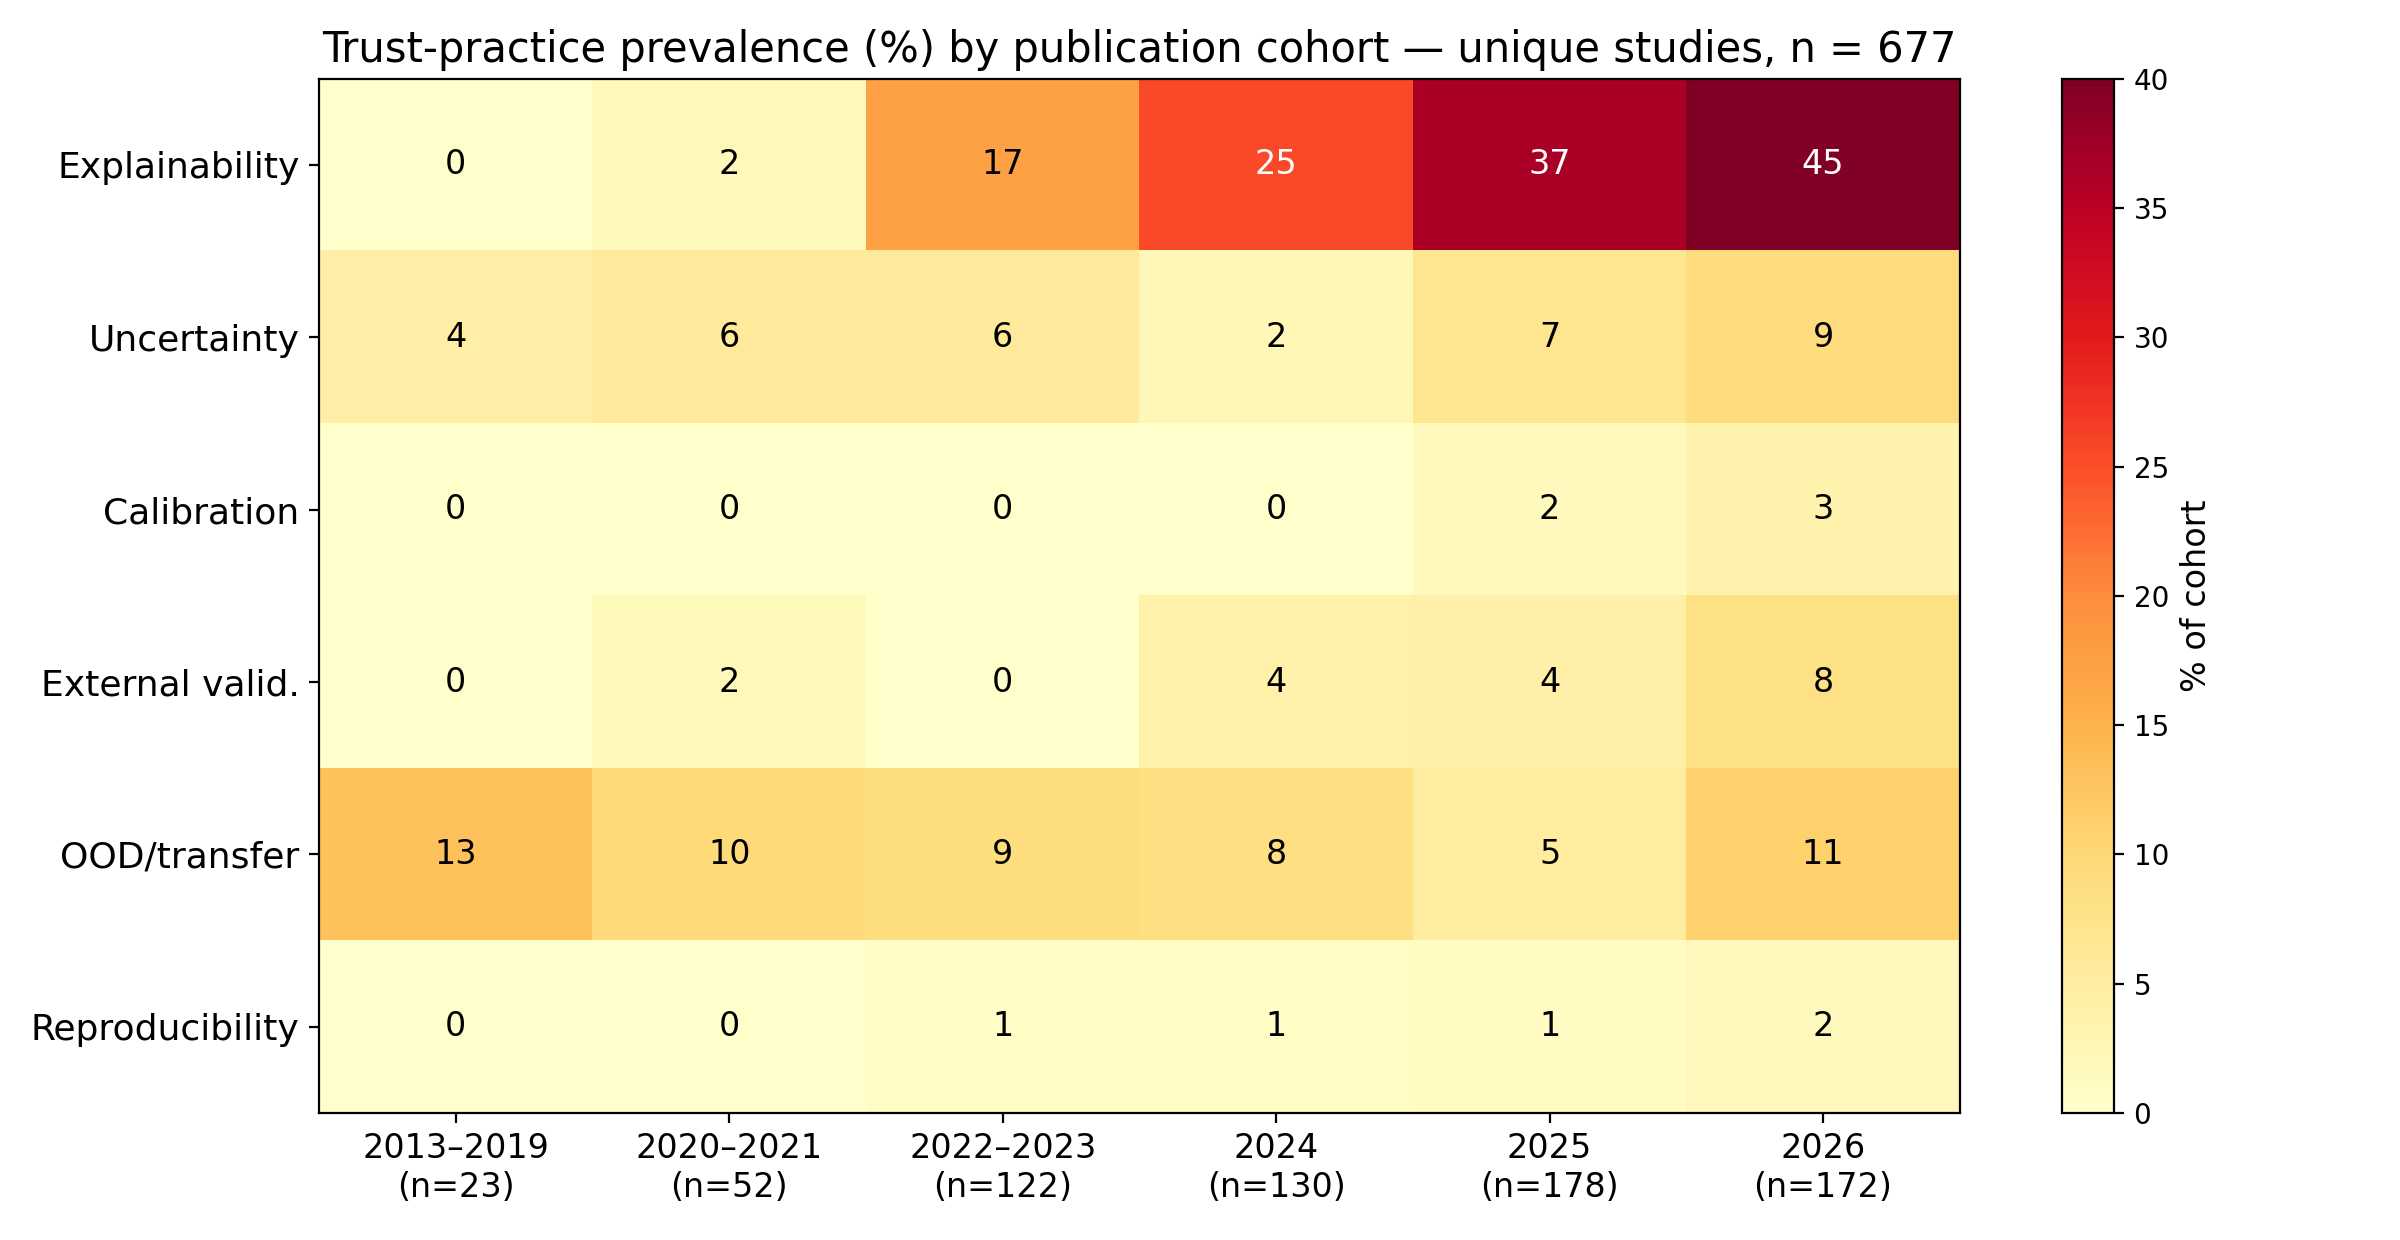
\includegraphics[width=0.95\textwidth]{Fig4.png}
\caption{Trust-practice prevalence by publication cohort: explainability diffuses; reliability practices do not. Cohort denominators shown on the axis (early cohorts are small; single studies move early-cohort values by several points)}\label{fig4}
\end{figure}

\begin{table}[htbp]
\caption{The trustworthy-AI scorecard: dimensions, operational questions, and corpus-wide prevalence (n = 677; title--abstract--keyword detection --- lower bounds; robustness and physical consistency were codable only in the full-text deep tier)}
\centering
{\footnotesize
\begin{tabular}{p{0.207\textwidth}p{0.517\textwidth}p{0.114\textwidth}l}
\toprule
Scorecard dimension & Core question & Studies (n) & \% of 677 \\
\midrule
XAI & Why did the model predict this? & 197 & 29.1 \\
UQ & How uncertain is the prediction? & 42 & 6.2 \\
calibration & Is stated confidence meaningful? & 9 & 1.3 \\
robustness & Stable under perturbation? (deep tier only) & 0 & 0.0 \\
OOD/transfer & Does it survive unseen chemistry? & 58 & 8.6 \\
external validation & Was genuinely independent data used? & 27 & 4.0 \\
physical consistency & Are outputs chemically plausible? (deep tier only) & 0 & 0.0 \\
reproducibility & Could another group repeat this? & 7 & 1.0 \\
none detected & No trust practice on any dimension & 407 & 60.1 \\
\bottomrule
\end{tabular}}
\end{table}

\section{Physics- and Chemistry-Informed AI: Auditing the Claims, Mapping the Frontier}

\subsection{A five-level scale and a conservative audit}

"Physics-informed" has become one of the most valuable labels in scientific machine learning, and correspondingly one of the most abused. To make claims commensurable, every study in the corpus was graded on a five-level integration scale: Type I, purely data-driven; Type II, domain quantities (oxide contents, Si/Al and Ca/Si ratios, activator moduli) included as ordinary input features; Type III, domain knowledge structurally shaping the model (knowledge graphs, chemistry-guided feature construction or architecture); Type IV, constrained learning, in which governing relations enter the loss or architecture (embedded equations, PINN formulations); and Type V, hybrid mechanistic--ML models coupling learning to thermodynamic or kinetic simulation. Assignment was conservative --- ambiguity resolves downward --- and, critically, \emph{claimed} labels were audited against what the methods actually do rather than accepted.

\subsection{The inflation finding}

At corpus scale, the P-axis distribution partitions by \emph{claim status}: 78.0\% [95\% CI 74.7--80.9] of studies are Type I and a further 18.0\% [15.3--21.1] Type II by demonstrated content (their sum, 96.0\%, is robust though the I-versus-II boundary is abstract-sensitive; Table S9), while the remaining 4.0\% --- twenty-seven studies --- merely \emph{claim} Type III or higher, with verification the subject of this section's audit. Partitioned instead by demonstrated content, assigning the fourteen deflated claims to their verified Types I--II, \textbf{98.1\% [96.7--98.9] of the corpus operates at Type II or below}; including oxide chemistry as features is now routine, and it is the full extent of "chemistry awareness" for nearly all of the field. Twenty-seven unique studies claim more (10 knowledge-guided, 7 physics-informed, 10 mechanistic-hybrid candidates; a twenty-eighth claim record proved to be a duplicate report and is excluded from the denominator --- Table 4 lists all 28 rows with the duplicate flagged). Auditing every one of the 27 claims produced the review's most uncomfortable quantitative result: \textbf{half of all physics- and chemistry-informed claims --- 14 of 27 (52\% [34.0--69.3]) --- do not survive scrutiny}. Nine claims verified at Type III or above; fourteen deflated to Types I--II, their "chemistry-informed" content amounting to oxide-ratio features, domain-informed feature priors, or a domain-motivated dataset; and four could not be verified from the available reporting, including one abstract whose dense stack of trending terms (transformer-PINN, spatiotemporal graph networks, embedded constraints) is asserted without a single specified constraint --- the pattern a skeptical reader recognizes as keyword engineering. A representative deflation is a "chemistry-informed" deep learner whose chemistry consists of adding oxide-ratio features to the input vector --- legitimate and useful feature engineering, but Type II, and materially different from what the label promises; per-study grades and rationales are released in Table 4 rather than singled out here. This inflation is not merely terminological. It corrupts evidence synthesis (a reader counting abstracts would overestimate the field's physics integration several-fold), and it devalues the label for the minority of studies that earn it. The audit table, released in full (Table 4), is intended as a reusable instrument: the Type scale plus the claimed-versus-verified discipline transfers directly to neighboring materials-AI literatures.

\subsection{The verified frontier: nine papers, five mechanisms, six years}

The genuine frontier is small enough to describe exhaustively --- the nine audit-verified studies, 1.3\% [0.7--2.5] of the corpus --- and it is real, mechanistically diverse, and strictly recent. (An earlier count of "roughly ten" reflected the duplicate report noted above; every frontier member both claimed and verified at Type III or higher. The audit covers claim-flagged studies by design, and the reliability recode surfaced one to two candidate mechanistic couplings the claim screen had not flagged --- Table S9 --- so, like every abstract-level count in this review, the frontier is a floor rather than a ceiling.) Its timeline is itself informative. Hybrid mechanistic coupling arrives first: machine learning joined to GEMS thermodynamic simulation to build composition--property relations across heterogeneous aluminosilicates (2021) \citep{ke2021}, followed by a random-forest formulation constrained simultaneously by network-topology and thermodynamic phase information across twenty-six precursors --- notably, the frontier's most transferability-oriented design \citep{bhat2022} --- and, in 2025, a chemistry-integrated ML framework coupling learning to thermodynamic modelling for one-part AAM strength development. Structural knowledge guidance appears next: a knowledge-graph-guided pipeline steering learning and multi-objective search for ultra-high-performance geopolymer (2024); a knowledge-graph-guided interpretable ensemble for geopolymer-stabilized dredged sludge, validated in situ (2025); and, in 2026, large-language-model automation that compresses knowledge-graph construction from $\sim$52 hours to $\sim$1 hour --- incidentally the corpus's first and only LLM touchpoint, firmly in a design-support rather than agentic role \citep{jiang2026}. Constrained learning arrives last and remains rarest: a carbonation-depth network with an embedded symbolic physical relation and dropout uncertainty (2025) \citep{liu2025}; physics-informed neural networks solving the inverse chloride-diffusion problem in alkali-activated mortars, where the PDE structure is the model (2025); and an equation-embedded network serving as the objective inside a four-objective evolutionary search over strength, cost, CO$_2$, and energy (2026) \citep{guo2026} --- the single study in 677 that simultaneously occupies the physics, design, and environmental axes, and thus the closest existing approximation to the trajectory's integrated endpoint.

Two observations follow. First, the frontier's mechanisms are complementary rather than competing --- thermodynamic hybrids supply phase realism, knowledge graphs supply relational structure, embedded constraints supply feasibility guarantees --- yet no study combines two of them. Second, the frontier is where transferability lives: the constrained and hybrid designs are precisely those reporting meaningful cross-precursor behavior, consistent with the physical argument that constraints substitute for the data the field does not have.

\subsection{What blocks diffusion}

Three causes recur. The dual-competence problem: embedding geopolymerization chemistry into learning requires fluency in both, and the corpus's authorship network shows minimal overlap between its materials-science and ML-methods clusters. The incentive problem: a Type II model with a fashionable label publishes as easily as a Type IV model that took a year longer to build --- this review's audit discipline is a small counter-incentive. And the benchmark problem: without shared datasets carrying reaction-relevant descriptors (amorphous content, reactive fractions, calorimetry), there is little for constraints to bind to (G6). The roadmap therefore couples terminology discipline (I4) with physics-constrained surrogates inside design loops (E1), validated by constraint-violation audits and ablations that isolate the physics contribution --- the evidentiary standard the current literature almost never meets.

\begin{figure}[htbp]
\centering
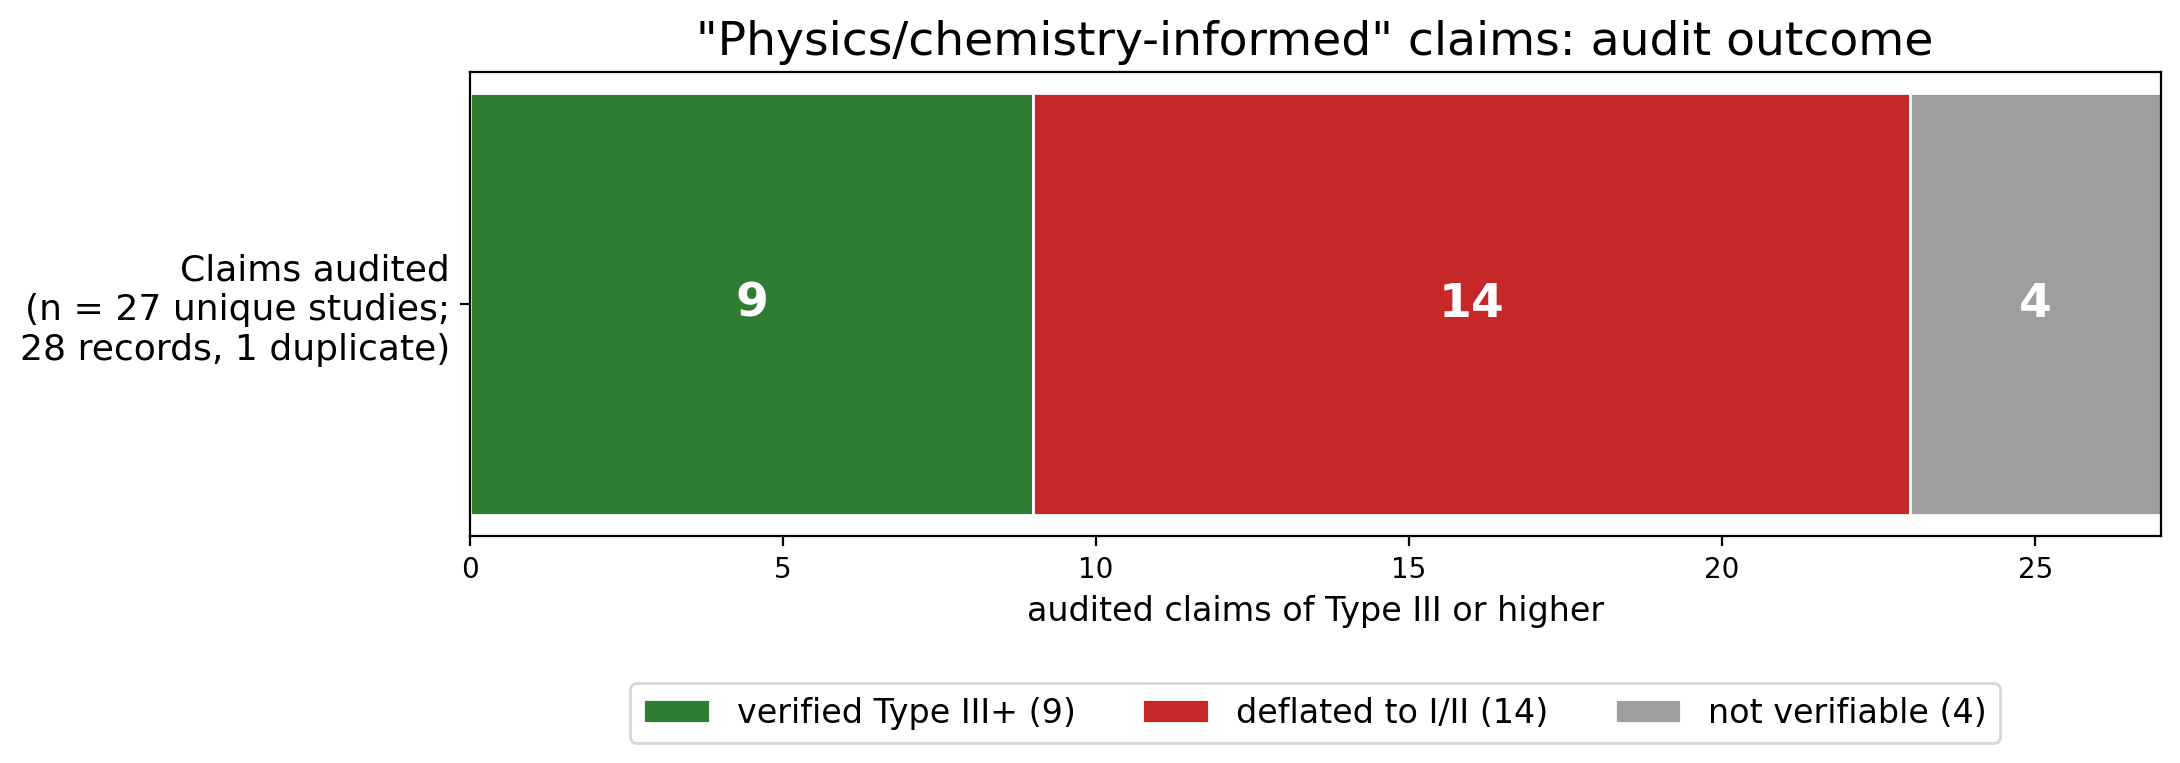
\includegraphics[width=0.95\textwidth]{Fig5.png}
\caption{Audit outcome of physics- and chemistry-informed claims: 27 unique claiming studies (28 claim records; one duplicate report excluded); 9 verified at Type III+, 14 deflated to Types I--II, 4 not verifiable}\label{fig5}
\end{figure}

{\footnotesize
\begin{longtable}{p{0.157\textwidth}p{0.052\textwidth}p{0.095\textwidth}p{0.615\textwidth}}
\caption{Claimed-versus-verified physics-integration audit: per-study grades (28 claim records = 27 unique claiming studies + 1 flagged duplicate report)}\\
\toprule
DOI & Claimed & Verified & Audit note \\
\midrule
\endfirsthead
\toprule
DOI & Claimed & Verified & Audit note \\
\midrule
\endhead
\bottomrule
\endfoot
\url{10.1007/s43939-026-00821-1} & III-claimed & II-verified & oxide ratios as input features only; "chemistry-informed" = feature choice \\
\url{10.1016/j.cemconcomp.2024.105723} & III-claimed & III-VERIFIED & knowledge graph structurally guides ML + MOO (strength/cost/carbon); genuine knowledge-guided design \\
\url{10.1016/j.wasman.2025.115139} & V-candidate & V-loose & ML and DFT run in parallel; DFT interprets, does not constrain the model \\
\url{10.1016/j.conbuildmat.2026.146774} & IV-claimed & I/II-verified & no physics; GP-guided boundary augmentation - BUT best OOD protocol in corpus (18\% out-of-range test) \\
\url{10.1007/s42107-026-01647-1} & V-candidate & I-verified & mechanisms motivational only; plain 4-model comparison \\
\url{10.1016/j.jobe.2024.110295} & V-candidate & II-verified & mechanism from experiments/characterization; ML is feature analysis \\
\url{10.1016/j.cemconcomp.2025.106364} & III-claimed & V-VERIFIED & CIML: ML integrated with thermodynamic modelling for one-part AAM \\
\url{10.1007/s40996-026-02191-3} & IV-claimed & UNVERIFIED-FT & physics entry point unclear from abstract; likely inflation \\
\url{10.1016/j.jclepro.2024.143974} & V-candidate & II-verified & ML clusters AE signals; physics via measurement not model \\
\url{10.1016/j.jobe.2025.113820} & IV-claimed & IV-VERIFIED & PINN solves inverse diffusion problem (PDE-constrained) for chloride Dc \\
\url{10.1016/j.autcon.2025.106667} & III-claimed & III-VERIFIED & LLM-automated knowledge-graph construction (52h to 1h) applied to UHPG design - FIRST LLM TOUCHPOINT IN CORPUS \\
\url{10.1007/s10973-026-15494-4} & V-candidate & I/II-verified & thermal experiments + predictive ML; no mechanistic coupling \\
\url{10.1038/s41598-025-27229-w} & IV-claimed & CLAIMED-FT-SKEPTICAL & TPINN+ST-GNN multi-degradation; buzzword density high, constraints unspecified - hostile-reviewer flag \\
\url{10.11591/ijict.v14i3.pp822-829} & IV-claimed & UNVERIFIABLE & abstract nearly content-free; quality concern \\
\url{10.1016/j.engappai.2025.113254} & III-claimed & IV-VERIFIED & KENN: governing equations embedded in NN + NSGA-II over strength/cost/CO2/energy \\
\url{10.1016/j.cscm.2025.e05407} & V-candidate & II-verified & multi-output RF; notable: embodied carbon as predicted output (885 mixes) \\
\url{10.1016/j.aei.2025.103982} & III-claimed & III-VERIFIED & knowledge graph guides variable selection + interpretation (PMV-IEL) \\
\url{10.12989/scs.2025.56.6.499} & V-candidate & II-verified & GMM phase clustering of nanoindentation data \\
\url{10.1016/j.conbuildmat.2021.126103} & III-claimed & II/III-verified & chemistry-based feature engineering (the 2022 paper that popularized the label) \\
\url{10.1016/j.compositesb.2021.108801} & V-candidate & V-VERIFIED & ML + global sensitivity + GEMS thermodynamics (2021 - earliest Type V) \\
\url{10.1016/j.conbuildmat.2022.127557} & V-candidate & IV/V-VERIFIED & RF with topological-network + thermodynamic constraints, 26 precursors \\
\url{10.1016/j.conbuildmat.2023.131519} & V-candidate & I/II-verified & plain RF; mechanisms motivational \\
(dup-AEI-row) & III-claimed & DUPLICATE & fallback duplicate of 10.1016/j.aei.2025.103982 with mismatched abstract - data note \\
\url{10.1016/j.cscm.2025.e05311} & IV-claimed & IV-VERIFIED & symbolic physics formula embedded in ANN + dropout UQ; abstract-level verification 31 Aug 2026 (referee-response audit extension) \\
\url{10.1016/j.dibe.2026.100951} & III-claimed & II-verified & "domain-informed features" = binder-chemistry inputs only; audit extension 31 Aug 2026 \\
\url{10.1007/s43452-025-01190-x} & IV-claimed & I-verified & VAE/GAN augmentation + MLP; no physics constraint anywhere in pipeline; audit extension 31 Aug 2026 \\
\url{10.1016/j.dibe.2026.100971} & III-claimed & II-verified & "domain-informed" AGP = feature priors + early-age posterior updating; no structural knowledge; audit extension 31 Aug 2026 \\
\url{10.1016/j.dibe.2025.100736} & III-claimed & II-verified & "chemistry-informed" CNN = oxide-composition input features; audit extension 31 Aug 2026 \\
\end{longtable}}

\section{Multi-Objective Optimization and Inverse Design: The Field's Real Advance, Half-Coupled}

\textbf{The honest revision to the thesis.} The hypothesis this review tests characterizes the field as prediction-centric, and Section 7 largely confirms it --- but a genuine design-search cluster now runs atop the surrogates. Its size requires care: 34.0\% [95\% CI 30.5--37.6] of the corpus carries the optimization label, but both independent reliability recodes (Table S9) show that label absorbing metaheuristic hyperparameter tuning as well as design-space search, so the demonstrated design cluster is better estimated at roughly 10--17\% of the corpus, floored by the 5.0\% explicitly multi-objective and 1.8\% inverse-design work --- still a real advance over the field the prior reviews described. The field has genuinely moved from "what strength will this mix have?" toward "what mix satisfies these requirements?" That advance deserves recording as such: design-space search is the trajectory's fourth stage, and the field occupies it. The audit finding is about what the search is coupled to.

\textbf{Anatomy of the design cluster.} Single-objective work maximizes strength, typically via genetic or swarm search over a fitted surrogate, and inherits every validity limitation of Section 15 --- an optimizer is an engine for finding the regions where a model is most wrong, and without applicability-domain guards (present in almost no study) its "optima" concentrate exactly where extrapolation is least trustworthy. Multi-objective work is more interesting and splits by objective set: strength--cost; strength--workability--durability; and the environmentally coupled frontier --- twenty-five studies across 2021--2026 placing carbon (occasionally energy) inside the objective vector (nineteen as their primary environmental treatment, six atop LCA or quantified emission-factor practice; Section 11.4 and Figure 6 reconcile the two counts), from an early generic framework optimizing environmental, financial, and mechanical criteria simultaneously \citep{shobeiri2022}, through NSGA-II and MOPSO treatments of fly-ash/slag systems, to 2025--2026 explainable-AutoML and stacked-ensemble variants. Inverse design proper --- from target properties to recommended formulations --- arrives through three routes: direct recommender systems with cost awareness \citep{natarajan2026}; generative approaches (VAE/GAN mix-repository construction \citep{gu2025}, with Section 18's caveats); and the corpus's most sophisticated exemplar, conformal-uncertainty-aware NSGA-II that returns \emph{design regions with reliability guarantees} rather than point optima, explicitly restricted to the model's applicability domain \citep{jagad2026}.

\textbf{The coupling deficit, precisely stated.} Across the cluster, three couplings that would make design outputs trustworthy are almost always absent --- uncertainty (Pareto fronts computed from point predictions, the conformal inverse-design exemplar \citep{jagad2026} excepted), physics (feasibility constraints beyond box bounds are rare; the single equation-embedded objective inside an evolutionary search \citep{guo2026} is the exception that proves the rule), and environmental assessment (the carbon terms optimized are unassessed emission-factor arithmetic; Section 11.3). And one coupling is absent everywhere: \emph{experiment}. No optimized mix reported as subsequently batched, tested, and fed back was detected anywhere in the coded corpus --- a zero checked against full-text deep extraction for the entire design cluster, not inferred from abstracts alone --- so design search remains an in-silico exercise whose recommendations end at a table. The cluster thus embodies the review's central pattern in miniature: capability demonstrated, trustworthiness deferred, loop never closed --- and its repair is correspondingly specific (roadmap E1--E2: constrained, uncertainty-aware, LCA-coupled search; F1: search that synthesizes).

\section{Environmental Performance, Carbon, and Life-Cycle Assessment: Claims Versus Quantification}

\subsection{Why this section is the review's center of gravity}

The scientific case for geopolymers is environmental: reuse of industrial residues and a substantially lower embodied carbon than Portland systems. Every AI study in this corpus inherits that motivation, and most repeat it. For a clean-technology assessment the operative question is therefore not whether the literature invokes sustainability but whether it \emph{quantifies} it --- with what data, what boundaries, and what uncertainty. The corpus was audited accordingly: every study coded for explicit environmental variables, and 76 studies --- every study whose abstract signals engagement with carbon, CO$_2$, or life-cycle assessment, whether as quantification or merely as framing, drawn from the 150 carbon/LCA-flagged unique studies --- individually classified on an evidentiary ladder from rhetoric to ISO-consistent assessment (Table 5). "Engagement" deliberately includes framing without quantification; that is what makes the ladder's bottom rung meaningful.

\subsection{The quantification pyramid}

The results form a steep pyramid. At corpus level, \textbf{44.8\% [95\% CI 41.1--48.5] of studies quantify no environmental variable at all} --- a figure the reliability recode marks as an undercount if anything, since a stricter reading of the quantification rule reclassifies more studies toward "none" than away from it (Table S9) --- in a literature whose titles and abstracts overwhelmingly advertise sustainable, green, eco-friendly, or low-carbon construction. Among the 76 environmentally engaged studies, 28\% remain framing-only even there. Ascending: 28\% quantify carbon through per-constituent emission factors --- a defensible screening practice, but one that imports generic, usually unreferenced, non-regionalized coefficients with no uncertainty; 25\% (19/76) carry carbon inside an optimization objective as their primary environmental treatment --- six further studies do so on top of LCA or emission-factor practice, giving the twenty-five-study design frontier of Section 11.4; 17\% perform something describable as an LCA; and \textbf{boundary-explicit, ISO-14040/44-consistent assessment appears in two studies --- approximately 0.3\% [0.1--1.1] of the corpus (2.6\% [0.7--9.1] even of the engaged 76)}. CO$_2$ uptake and mineralization, a headline argument for alkali-activated systems' environmental case, is essentially absent as a modeled quantity. The asymmetry deserves plain statement: the field's environmental claims scale with its publication count; its environmental evidence does not.

\subsection{The emission-factor economy and its consequences}

Deep extraction shows how the middle of the pyramid works. The dominant pattern computes a per-cubic-meter CO$_2$ footprint by multiplying mix quantities against literature emission factors, then either reports it \citep{alfakih2024} or optimizes against it. The practice has two structural weaknesses. First, factor provenance: sodium-silicate production factors in circulation vary severalfold depending on source and system boundary, and no audited study propagates that variation --- meaning optimizers may be trading strength against carbon differences smaller than the carbon data's own error. Second, circularity: when the CO$_2$ target is itself computed from mix proportions by fixed arithmetic, a model "predicting" it partially re-learns that arithmetic, and headline accuracies overstate environmental insight \citep{alfakih2024}. Where life-cycle framing does appear, it is typically cradle-to-gate with activator production dominating impacts --- a robust and repeatedly rediscovered result that the AI layer has yet to exploit systematically, for instance by treating activator demand as the primary design lever under uncertainty.

\subsection{The genuine frontier: twenty-five studies of environmentally objective design}

Set against this, the corpus contains a real and growing subfield --- twenty-five studies, 2021--2026, verified against the released audit table (19 with carbon-as-objective as primary treatment plus 6 combining it with higher-rung practice) --- in which environmental quantities enter the objective function rather than the discussion section. Its arc runs from a generic augmented mix-design framework optimizing environmental, financial, and mechanical criteria \citep{shobeiri2022}, through NSGA-II and particle-swarm frameworks trading strength, cost, and CO$_2$ for fly-ash/slag systems \citep{huang2023}, to 2025--2026 work coupling explainable ensembles and AutoML to multi-objective search over strength, durability, and carbon efficiency, and --- at the frontier's integrated best --- an equation-embedded network optimizing strength, cost, CO$_2$, \emph{and} energy simultaneously \citep{guo2026}. One foam-concrete study reports a carbon footprint of $\sim$139 kg CO$_2$/m$^3$ for its optimized mixture alongside a 19.7\% cost reduction \citep{song2026} --- the kind of jointly quantified claim this literature should normalize, though the figure rests on per-constituent emission factors within a cradle-to-gate frame, exactly the practice whose unpropagated uncertainty Section 11.3 cautions about. Three properties characterize the frontier at its best and expose the rest: carbon data with stated provenance, trade-offs presented as Pareto structure rather than single optima, and honest reporting when environmental and mechanical objectives conflict. Even here, however, factor uncertainty is unpropagated, boundaries stop at the gate, and no physically batched optimized "low-carbon" mix with a verified inventory was detected in the coded corpus (checked by full-text extraction across the audited 76) --- the validation requirement this review sets for the claim (Section 19, G4).

\subsection{Implications for a clean-technology journal}

For the venue of this review the conclusion is direct. AI has demonstrably learned to \emph{optimize} carbon numbers; the field has not yet earned the right to call the results low-carbon materials, because the numbers being optimized are unassessed. Closing that gap is cheaper than it appears --- regionalized inventories for the dominant precursors and activators, factor-uncertainty propagation into Pareto fronts, and an LCA-disclosure norm for sustainability claims (Section 20, E2; Section 17) --- and the two ISO-grade studies prove it is publishable practice, not aspiration. Until then, the honest summary of AI's environmental contribution in geopolymer research is: rhetorically universal, arithmetically occasional, assessed almost never.

\begin{figure}[htbp]
\centering
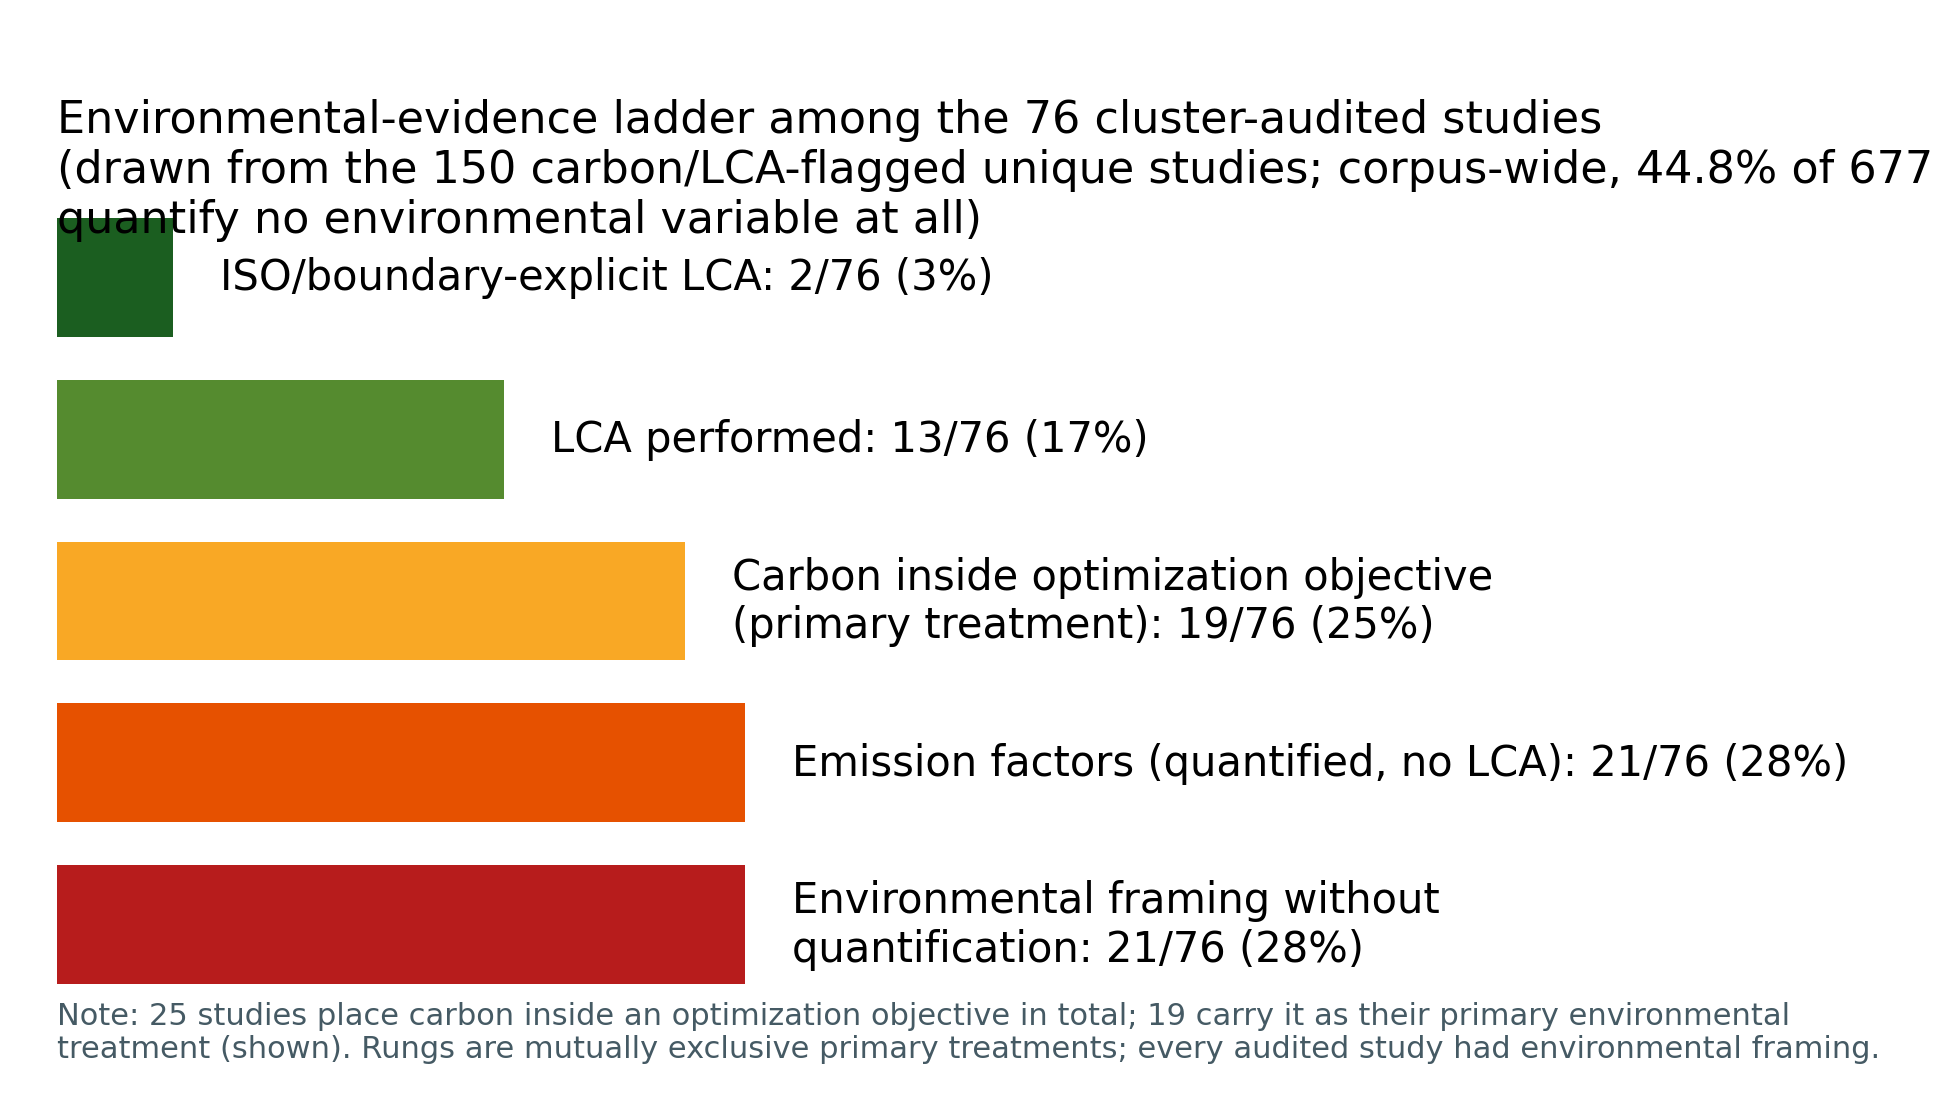
\includegraphics[width=0.95\textwidth]{Fig6.png}
\caption{The environmental-evidence ladder among the 76 environmentally engaged studies of the cluster audit (drawn from the 150 carbon/LCA-flagged unique studies). Rungs are mutually exclusive primary treatments; "engagement" includes framing without quantification, which is what makes the bottom rung meaningful. In total 25 studies place carbon inside an optimization objective (19 as primary treatment, shown)}\label{fig6}
\end{figure}

{\footnotesize
\begin{longtable}{p{0.326\textwidth}lp{0.267\textwidth}lp{0.188\textwidth}}
\caption{Carbon/LCA cluster audit: per-study evidentiary classification of the 76 environmentally engaged studies (full records incl. titles and venues in the released artifact)}\\
\toprule
DOI & Year & Primary carbon treatment & Quantified & Carbon in objective \\
\midrule
\endfirsthead
\toprule
DOI & Year & Primary carbon treatment & Quantified & Carbon in objective \\
\midrule
\endhead
\bottomrule
\endfoot
\url{10.1016/j.jclepro.2025.147176} & 2025 & carbon-as-objective & N & Y \\
\url{10.3390/ma17205086} & 2024 & rhetoric-only & N & N \\
\url{10.1016/j.mtcomm.2025.112326} & 2025 & carbon-as-objective & N & Y \\
\url{10.1016/j.clwas.2025.100270} & 2025 & emission-factors-quantified & N & N \\
\url{10.1016/j.istruc.2026.111649} & 2026 & LCA-performed & N & N \\
\url{10.1007/s42107-025-01450-4} & 2025 & carbon-as-objective & N & Y \\
\url{10.1016/j.jobe.2026.115878} & 2026 & emission-factors-quantified & Y & N \\
\url{10.1080/14680629.2025.2495705} & 2026 & LCA-performed & Y & N \\
\url{10.1061/JSDCCC.SCENG-2032} & 2026 & emission-factors-quantified & Y & N \\
\url{10.1016/j.jclepro.2024.143463} & 2024 & carbon-as-objective & N & Y \\
\url{10.1016/j.rinma.2025.100791} & 2025 & carbon-as-objective & Y & Y \\
\url{10.1016/j.jclepro.2026.147501} & 2026 & carbon-as-objective & N & Y \\
\url{10.1038/s41598-026-48502-6} & 2026 & LCA-performed & N & Y \\
\url{10.1016/j.powtec.2025.121900} & 2026 & emission-factors-quantified & N & N \\
\url{10.32604/cmes.2026.083654} & 2026 & emission-factors-quantified & N & N \\
\url{10.18702/acf.2025.11.1.53} & 2025 & rhetoric-only & N & N \\
\url{10.3390/ma19112235} & 2026 & rhetoric-only & N & N \\
\url{10.1038/s41598-025-27361-7} & 2025 & carbon-as-objective & N & Y \\
\url{10.1016/j.cemconcomp.2024.105723} & 2024 & rhetoric-only & N & N \\
\url{10.3390/su17167483} & 2025 & LCA-performed & Y & N \\
\url{10.1007/s42107-025-01367-y} & 2025 & emission-factors-quantified & N & N \\
\url{10.1007/s42107-025-01506-5} & 2026 & rhetoric-only & N & N \\
\url{10.1007/s42107-026-01700-z} & 2026 & emission-factors-quantified & N & N \\
\url{10.1061/JSDCCC.SCENG-1724} & 2025 & emission-factors-quantified & N & N \\
\url{10.1016/j.eswa.2026.133523} & 2027 & carbon-as-objective & N & Y \\
\url{10.54740/ros.2026.024} & 2026 & emission-factors-quantified & Y & N \\
\url{10.3390/infrastructures11040138} & 2026 & carbon-as-objective & Y & Y \\
\url{10.1016/j.hybadv.2025.100569} & 2025 & rhetoric-only & N & N \\
\url{10.1515/rams-2025-0249} & 2026 & emission-factors-quantified & N & N \\
\url{10.3390/buildings16010123} & 2026 & rhetoric-only & N & N \\
\url{10.1002/suco.70211} & 2025 & emission-factors-quantified & N & N \\
\url{10.1016/j.oceram.2025.100861} & 2025 & ISO/boundary-LCA & Y & N \\
\url{10.1016/j.clema.2024.100258} & 2024 & emission-factors-quantified & N & N \\
\url{10.1371/journal.pone.0336654} & 2026 & LCA-performed & Y & Y \\
\url{10.1007/s43621-025-02447-4} & 2026 & LCA-performed & Y & N \\
\url{10.3390/buildings15122081} & 2025 & LCA-performed & Y & Y \\
\url{10.1016/j.jece.2025.119847} & 2025 & LCA-performed & Y & N \\
\url{10.1016/j.conbuildmat.2025.144257} & 2025 & rhetoric-only & N & N \\
\url{10.1016/j.advengsoft.2024.103611} & 2024 & rhetoric-only & N & N \\
\url{10.1080/10589759.2024.2334434} & 2025 & carbon-as-objective & N & Y \\
\url{10.1007/s00500-025-10710-z} & 2025 & rhetoric-only & N & N \\
\url{10.1016/j.powtec.2025.122082} & 2026 & rhetoric-only & N & N \\
\url{10.3390/ma17143540} & 2024 & emission-factors-quantified & N & N \\
\url{10.1016/j.aei.2025.103982} & 2026 & emission-factors-quantified & Y & N \\
\url{10.3390/ma19102168} & 2026 & rhetoric-only & N & N \\
\url{10.1371/journal.pone.0310422} & 2024 & LCA-performed & Y & Y \\
\url{10.1016/j.rineng.2024.102158} & 2024 & emission-factors-quantified & Y & N \\
\url{10.3390/buildings14123998} & 2024 & emission-factors-quantified & N & N \\
\url{10.1038/s41598-024-54513-y} & 2024 & rhetoric-only & N & N \\
\url{10.1016/j.mtcomm.2024.109599} & 2024 & carbon-as-objective & N & Y \\
\url{10.1061/JMCEE7.MTENG-23191} & 2026 & emission-factors-quantified & Y & N \\
\url{10.1038/s41598-026-44832-7} & 2026 & LCA-performed & N & N \\
\url{10.1007/s00521-025-11191-9} & 2025 & carbon-as-objective & Y & Y \\
\url{10.1038/s41598-025-18666-8} & 2025 & carbon-as-objective & Y & Y \\
\url{10.1016/j.conbuildmat.2025.144380} & 2025 & carbon-as-objective & N & Y \\
\url{10.1016/j.rineng.2025.105537} & 2025 & rhetoric-only & N & N \\
\url{10.28991/CEJ-2025-011-04-020} & 2025 & rhetoric-only & N & N \\
\url{10.1038/s41598-026-43052-3} & 2026 & LCA-performed & N & N \\
\url{10.1007/s10668-025-06957-z} & 2025 & carbon-as-objective & Y & Y \\
\url{10.1016/j.conbuildmat.2024.136013} & 2024 & carbon-as-objective & N & Y \\
\url{10.1016/j.jobe.2023.106577} & 2023 & carbon-as-objective & N & Y \\
\url{10.1016/j.jobe.2023.106929} & 2023 & emission-factors-quantified & Y & N \\
\url{10.12989/scs.2022.45.6.877} & 2022 & rhetoric-only & N & N \\
\url{10.3390/su16010142} & 2024 & rhetoric-only & N & N \\
\url{10.3390/su13137444} & 2021 & emission-factors-quantified & Y & N \\
\url{10.1080/21650373.2024.2416962} & 2024 & rhetoric-only & N & N \\
\url{10.1016/j.jclepro.2022.133382} & 2022 & LCA-performed & Y & Y \\
\url{10.1016/j.measurement.2022.111916} & 2022 & emission-factors-quantified & N & N \\
\url{10.3390/app10217726} & 2020 & emission-factors-quantified & N & N \\
\url{10.1016/j.jece.2023.111835} & 2024 & carbon-as-objective & N & Y \\
\url{10.3390/ma14092401} & 2021 & ISO/boundary-LCA & N & Y \\
\url{10.3390/su14159573} & 2022 & LCA-performed & Y & N \\
\url{10.1016/j.jobe.2023.106070} & 2023 & carbon-as-objective & N & Y \\
\url{10.12989/scs.2024.50.4.443} & 2024 & rhetoric-only & N & N \\
\url{10.3390/ma13235490} & 2020 & rhetoric-only & N & N \\
\url{10.1016/j.conbuildmat.2023.131519} & 2023 & rhetoric-only & N & N \\
\end{longtable}}

\section{AI for Industrial-Waste Valorization: Modeling the Easy Streams}

Waste valorization is the circularity half of the geopolymer promise, and 28\% of the corpus engages it at least nominally. The engagement is real but asymmetric in the same direction as Section 6: streams with standardized supply chains and abundant published data (fly ash, GGBFS) are modeled hundreds of times, while the environmentally urgent, chemically difficult streams --- red mud (1.0\% of studies), mine tailings (1.1\%), municipal and incineration residues, dredged and excavated sediments --- appear in dozens at most. Yet it is precisely these hard streams where the corpus's most instructive valorization work happens, because their variability forces methodological honesty that easy streams never demand.

Three patterns characterize the frontier. First, \textbf{reactivity-centered modeling}: rapid ML classification of coal fly-ash reactivity for recycling triage \citep{qi2022}, and a PCA-based framework assessing fifteen heterogeneous solid wastes before prediction \citep{song2025} --- studies that treat feedstock characterization as the modeling problem, rather than assuming composition suffices. Second, \textbf{multi-waste synergy design}: ternary and all-solid-waste systems (fly ash--slag--steel slag; slag--gangue; sludge--silica fume) where ML untangles interaction effects that factorial experimentation cannot afford, occasionally with knowledge-guided variable selection \citep{su2026}. Third, \textbf{environmental-function coupling}: heavy-metal solidification/stabilization models for incineration fly ash and coal-gangue systems --- including the corpus's lone ML+DFT pairing, which interrogates immobilization mechanisms alongside prediction --- where the modeled target \emph{is} the environmental service, closing the gap between valorization rhetoric and quantified function that Section 11 criticizes elsewhere.

The strategic reading for a clean-technology audience: as decarbonization shrinks the easy streams (Section 3), the field's data assets depreciate while its hard-stream capabilities remain embryonic. The valorization agenda therefore converges with the review's data agenda --- regional characterization datasets carrying reactivity descriptors for tailings, red mud, and emerging residues (G6, roadmap I1/E2) --- and with its transfer agenda, since models robust across variable feedstocks are exactly what Section 9's constrained approaches promise and Section 15's evaluation practices would certify.

\section{Digital Twins and Adaptive Material Models: Ingredients Without Assembly}

No construction of a digital twin of a geopolymer material, process, or structure was detected anywhere in the coded corpus --- a zero established not by coding absence alone but by a dedicated search arm: Scopus query family F targeted "digital twin" and autonomy terms directly (180 records), and its geopolymer-relevant yield was empty --- against a construction-informatics literature where the term is ubiquitous. What the corpus does contain --- dispersed and unassembled --- are the twin's components. State sensing: in-situ acoustic-emission monitoring of early-age alkali-activated reaction, machine-clustered into physically interpretable stages. State models: PINN-identified transport coefficients (chloride diffusion) and carbonation-depth models with embedded physics (Section 9) --- precisely the degradation kernels a service-life twin would run. State updating: the amortized Gaussian-process framework that revises later-age strength predictions from early-age observations with calibrated uncertainty \citep{chan2026} --- functionally, a data-assimilation step awaiting a loop to live in. And interface precedents: the design GUIs and recommender systems of Section 10, which are twins' decision-support layer without their synchronized physical counterpart.

Why assembly has not happened is largely Section 14's story (tempo, heterogeneity, incentive structure), but one twin-specific obstacle deserves note: a twin needs a \emph{thing} to mirror, and the corpus's models mirror datasets, not instrumented specimens or elements. The shortest credible path, argued in the roadmap (F2), is deliberately modest --- one instrumented pilot element, one assimilation loop joining monitoring stream to physics-informed degradation model to updating predictor, one published comparison of twin-predicted versus measured indicators. The components above make that a systems-integration project rather than a research gamble, which is exactly what their scattered existence indicts: the field has built the parts of a capability it has never once assembled.

\section{Adaptive Experimentation and Autonomous Discovery: A Stage Awaiting Its First Loop}

\subsection{Scope and evidentiary discipline}

This section evaluates the trajectory's upper stages --- active and sequential learning, digital twins, foundation models and language-model agents, and closed-loop autonomous discovery --- under a rule applied nowhere else in this literature: every capability claim is graded as demonstrated in geopolymers, demonstrated only in adjacent materials science, or prospective, and adaptive workflows are explicitly sub-coded as \emph{simulated} (retrospective selection from an already-measured pool) versus \emph{physical} (new syntheses inside the loop). The rule matters because this is the region of the trajectory where enthusiasm most outruns evidence.

\subsection{Adaptive experimentation: three studies, all simulated}

Sequential and active learning --- the machinery that turns a predictor into an experiment-planner --- appears in exactly three of 677 unique studies (0.4\% [95\% CI 0.2--1.3]); an earlier count of four included a duplicate report of the active-learning UHPC study, caught and flagged by the synthesis duplicate audit (Section 2.6). The lineage begins in 2021 with sequential learning over a 131-mixture alkali-activated binder space, benchmarking Gaussian-process and tree-ensemble surrogates under several acquisition functions and reporting that the experiments required to reach a target strength can fall by roughly an order of magnitude relative to model-free search \citep{volker2021}. A 2023 successor scales the benchmark to eight curated datasets and, significantly for this review, injects CO$_2$ footprints as a co-objective, showing that sequential learning can navigate strength--carbon trade-offs with small initial datasets \citep{volker2023}. A 2025 study wraps active learning around stacked ensembles for alkali-activated UHPC, reporting modest but real accuracy gains ($\approx$4 percentage points) and --- uniquely in this cluster --- spot-validating its tuned model against newly performed laboratory tests through a released design interface \citep{kazemi2025}. The common denominator: in every case the "experiments" selected by the algorithm were rows in an existing database. The loop that defines the method --- propose, synthesize, measure, update --- has never once been closed physically in this material system. The honest summary is that geopolymer research possesses simulated evidence that adaptive design \emph{would} work, and no evidence that anyone has \emph{done} it.

\subsection{Digital twins: absence established, components inventoried in Section 13}

Digital twins are absent as assembled systems --- the zero established by dedicated search, and the scattered components (acoustic-emission state sensing \citep{jin2024}, physics-informed degradation kernels, posterior-updating strength prediction \citep{chan2026}) inventoried in Section 13, which also specifies the shortest assembly path (roadmap F2). The absence matters here because it interacts with autonomy: the posterior-updating enabler that Section 13 identifies is the same machinery that addresses the 28-day tempo problem breaking loop iteration for any adaptive or autonomous scheme (Section 19, G5).

\subsection{Foundation models and language agents: a 2026 arrival, in a support role}

Two 2026 studies mark the entry of the foundation-model era into this literature, and their roles deserve precise statement. A tabular foundation model (TabPFN variant) with episodic training targets the extrapolation problem directly, evaluated under a dedicated out-of-range protocol \citep{zhang2026}; and a large-language-model pipeline automates construction of materials knowledge graphs --- compressing an expert task from days to an hour --- which then guide design for ultra-high-performance geopolymer \citep{jiang2026}. Both are design-support tools operated by humans. No scientific agent that plans geopolymer experiments, no LLM-driven laboratory orchestration, and no autonomous hypothesis generation was detected --- a zero checked by the dedicated autonomy search arm (query family F: "AI agent", "agentic", "autonomous laboratory", "self-driving laboratory", "closed-loop experiment"; 180 records, none geopolymer-eligible) in addition to the corpus coding; against the master framing of this review, "agentic AI" in geopolymer research is at present a null set, and this paper deliberately confines the term to its roadmap (Section 20, F3).

\subsection{The adjacent-domain contrast and the transfer barriers}

The emptiness is not for want of exemplars next door. Self-driving laboratories now run closed loops routinely in molecular materials, thin films, and formulation chemistry, with mature reviews of both the technology and its governance \citep{tom2024}. Why has none of it crossed into alkali-activated binders? Deep extraction and domain analysis converge on four barriers: verification tempo (mechanical targets mature over 28 days; loop iteration time is the killer variable); feedstock heterogeneity (industrial residues vary batch-to-batch in ways that break the fixed protocol assumption of current SDL stacks); handling (viscous silicate activators and paste rheology are less robot-friendly than solution chemistry --- though one-part dry-mix formulations largely dissolve this barrier, motivating the roadmap's choice of entry point); and the validation deficit itself (an autonomous loop steered by uncalibrated surrogates compounds Section 8's problems at machine speed). None of these barriers is fundamental; all four have engineering answers already present, scattered, inside the corpus --- early-age surrogates for tempo, reactivity descriptors for heterogeneity, one-part systems for handling, conformal calibration for trust. Assembling them into one demonstration is the field's most consequential open experiment, and the roadmap specifies what its minimal credible version must show: at least two consecutive physical propose--synthesize--test--update cycles with declining, calibrated uncertainty (Section 20, F1).

\section{Benchmark, Validation, and Reproducibility: An Audit of the Field's Evidentiary Base}

\subsection{The dataset economy}

The corpus runs on recycled data. The dominant supply chain is the literature compilation: mixes and measured properties harvested from prior experimental papers into tabular databases of roughly one hundred to nine hundred records, which then circulate from study to study. Deep extraction repeatedly encountered the same compilations --- 594-, 672-, and 676-record databases among them --- under dozens of different models, and the pattern's consequences compound. First, effective sample size: fifty models tuned on the same six hundred rows constitute one study of a dataset, not fifty studies of a material. Second, contamination: the single audited case of database hygiene removed 37 duplicate records from a 594-record standard compilation before modeling \citep{parakhiya2026} --- duplicates that every prior user of that database had presumably trained and tested across, silently inflating scores. Third, invisibility: provenance is rarely machine-readable, so dataset reuse cannot even be tracked systematically; this review identified recirculation by matching record counts and source citations, a method that undercounts. The field's growth statistics (Section 4) must therefore be read carefully: publications grew tenfold since 2020; the underlying experimental evidence base grew far more slowly.

This review is not exempt from its own finding, and says so. The post-freeze duplicate audit of our corpus (Section 2.6) caught 52 duplicate reports --- 7.1\% of included records --- that title-abbreviation had slipped past a DOI-and-title merge, a rate of the same order as the 37-in-594 contamination documented above. The difference is not virtue but procedure: the audit existed, ran before synthesis statistics were finalized, and its pair-level evidence is released. That is precisely the provenance discipline whose absence in the field's compiled databases this section documents.

\subsection{Validation practice: one ladder, mostly unclimbed}

A deployment-relevant evaluation ladder runs: internal cross-validation $\rightarrow$ held-out test $\rightarrow$ external dataset $\rightarrow$ cross-laboratory $\rightarrow$ prospective (predict, then synthesize). Corpus practice concentrates overwhelmingly on the first rung, with random splits of compiled data; the invalid-comparison rule of Section 2 exists because papers routinely rank their R$^2$ against competitors' R$^2$ across different datasets, splits, and preprocessing --- a comparison with no evidentiary content. Rungs beyond the second are sparsely populated: external-validation signals appear in 4.0\% [2.8--5.7] of the corpus, and the audited genuinely independent designs are few enough to list (Section 8.4). On the two upper rungs, no interlaboratory study and no prospective validation was detected in the coded corpus --- an absence established at title--abstract level and additionally checked by targeted full-text search across the deep-extraction tier. One consequence is quantifiable optimism wherever honest degradation is reported --- cross-validated MAE of 6.23 MPa becoming 7.86 MPa on an independent test in the one decision-support system that reports both \citep{natarajan2026} --- and unquantifiable optimism everywhere it is not. A cheap corrective exists and has not been used: time-split meta-validation, training on pre-2024 literature and testing on the 2024--2026 flood, is executable today from published data alone and would give the field its first honest estimate of forward error (Section 20, I5).

\subsection{Leakage, near-duplicates, and the group problem}

Compiled databases carry a structural leakage risk that random splitting ignores: the same mix family --- one laboratory's factorial sweep, reported across several papers --- lands in both train and test folds, so the model is examined on near-copies of its training data. Only one audited study engineers against this, constraining identical feature-vector groups to single subsets \citep{parakhiya2026}; the applicability-domain analysis of its companion study then demonstrates what unbiased evaluation reveals --- that reported accuracy reflects dense interpolation within a structured experimental envelope \citep{jagad2026}. These two practices --- group-aware splitting and validity-domain declaration --- are standard in cheminformatics and medical ML; their near-total absence here is a portability failure of methodology, not a limitation of the material.

\subsection{Reproducibility: statements without artifacts}

Data-availability statements are now common; verifiable artifacts are not. Explicit code-availability signals were detectable in roughly one percent of the corpus at abstract level (7 of 677), while among the sixteen deep-extracted studies --- selected for being the field's methodological best --- not one stated a resolvable code repository in full text; the two figures measure different things (abstract signals versus verified resolvable artifacts) and together bound true code availability between approximately zero and one percent. Hyperparameters are reported inconsistently; preprocessing pipelines (imputation, outlier handling, normalization) are described in prose that rarely permits reconstruction. The field is thus in the position of asserting reproducibility norms it does not practice. A final integrity observation from this review's own process belongs on the record: the screening stage caught a retraction notice circulating in the corpus only through human dual review, and no mechanism exists by which retractions propagate into the compiled databases that downstream models train on --- a small but telling illustration of the provenance vacuum (Section 20, Section~5 governance).

\subsection{Synthesis}

The audit's conclusion is structural rather than accusatory: individually reasonable choices --- compile published data, split randomly, report R$^2$, move on --- aggregate into a field whose headline numbers cannot support the engineering decisions they invite. The three cheapest repairs (calibration reporting, group-aware splits with validity domains, and a FAIR benchmark with fixed splits and provenance) are the roadmap's immediate tier precisely because nothing about them requires new laboratories --- only new habits.

\section{From Laboratory Prediction to Clean-Technology Deployment: The Unbuilt Last Mile}

Coded on the deployment axis, the corpus's ceiling is low and sharply defined. The modal study ends at laboratory prediction. A substantial minority reaches formulation recommendation; a handful of decision-support tools and GUIs --- some experimentally spot-checked \citep{natarajan2026,kazemi2025} --- mark the field's most deployed artifacts. Above that, none of the following was detected in the coded corpus of 677 studies (title--abstract--keyword level, cross-checked against the full-text deep-extraction tier): a process-control implementation in a production setting, a pilot project reporting model-guided mix deployment, engagement with certification, or any appearance of the standards bodies whose acceptance any structural material must eventually win. The gap is not merely unfilled; it is unaddressed, as though deployment were another discipline's problem.

For this journal's remit the analysis must be structural. Construction-materials acceptance is prescriptive: codes specify compositions and procedures calibrated over decades of Portland practice, and a model's output --- a predicted property with (rarely) an uncertainty --- has no port of entry. The technically coherent bridge is performance-based acceptance, which several jurisdictions already permit in limited forms: acceptance criteria stated over measured performance plus a conformity-testing regime, into which a calibrated prediction interval fits naturally as a \emph{screening and design} instrument that reduces, but never replaces, physical verification. This is precisely where the trust deficits of Sections 8 and 15 become economic rather than academic: an uncalibrated model cannot tell a certifier how much physical testing its predictions warrant forgoing, so it warrants forgoing none, and its industrial value collapses to convenience. Conversely, the corpus's conformal exemplars show what a certifiable prediction would look like --- coverage-verified intervals with declared validity domains --- and no study has yet walked one through even a precast product approval, the lowest-friction entry point.

Deployment, then, is not a future stage of this field so much as its missing boundary condition: the requirement that would discipline model evaluation (Section 15), justify environmental quantification (Section 11), and give the roadmap's parallel track (D1--D3) its destination --- a documented case, at any scale, of an AI-designed alkali-activated mix accepted through a performance-based process. Until that case exists, the field's contribution to decarbonized construction remains, strictly speaking, hypothetical.

\section{Standards, Governance, and Implementation Pathways}

Five governance instruments follow from the audits, ordered by who can act.

\textbf{Journals and reviewers (actionable immediately).} First, a reporting checklist for AI studies on construction materials --- data provenance and availability, split design and leakage controls, validity-domain declaration, calibration metrics beside accuracy, environmental boundary statement, code release --- for which this review's scorecard and coding scheme constitute a working draft. Second, an environmental-claims disclosure norm: manuscripts asserting "low-carbon" or "sustainable" outcomes state their quantification basis (none / emission factors with sources / LCA with boundaries), a single required sentence that would have re-classified a quarter of this corpus's environmental rhetoric overnight. A journal positioned at the technology--policy interface, such as this one, could adopt both unilaterally and would set the field's norm by doing so.

\textbf{The research community (near-term).} Third, benchmark governance: the FAIR dataset of roadmap I1 requires stewardship --- versioning, duplicate policing, contribution credit, and retraction propagation. On the last point this review offers direct evidence of the vacuum: a retracted study was caught circulating toward the corpus only by human dual-screening, and nothing currently removes retracted results from the compiled databases on which the field trains. Data stewardship of this kind is unglamorous, fundable, and prerequisite to every quantitative claim the field will make.

\textbf{Standards bodies and regulators (structural).} Fourth, engagement of RILEM, ASTM, and CEN committees on the evidentiary status of model outputs within performance-based acceptance --- the specific question of how a coverage-verified prediction interval may substitute for a fraction of conformity testing, and under what validity-domain declarations. Fifth, digital material passports for AAM products binding feedstock provenance, oxide and reactivity characterization, life-cycle inventory, and model validity metadata --- an instrument that aligns naturally with emerging construction-products regulation and would make the traceability this review laboriously reconstructed a property of the material itself.

None of these instruments requires scientific novelty; all five require institutional will. Their absence, not any algorithmic limitation, is presently the binding constraint on AI's contribution to low-carbon construction --- which is why they run as a parallel track through the roadmap rather than as its final stage.

\section{Contradictions and Methodological Tensions Within the Field}

A synthesis that reports only convergence flatters its corpus. This section records where the literature disagrees with itself, because the disagreements delimit what is actually known (Table 6 summarizes the four tensions and their resolutions).

\textbf{Synthetic augmentation: the sharpest conflict.} The corpus's favorite remedy for small data is generative augmentation, and its evidence is contradictory at the level of direct opposition. One line of work reports that variational-autoencoder and GAN-generated samples, screened by a custom similarity check, enable a reliable mix-design framework for coal-gangue AAMs (R$^2$ $\approx$ 0.96) \citep{gu2025}; another, testing conditional tabular GAN augmentation within a carbonation-prediction framework, finds it \emph{degrades} accuracy and generalization relative to training without it \citep{liu2025}. Between these poles sit numerous studies --- Gaussian-noise augmentation, imputation-plus-augmentation pipelines, GP-guided boundary synthesis --- reporting benefits without testing a harm case. The contradiction is unresolved because the evaluations are incommensurable: synthetic data is typically scored on distributions derived from the same small samples that generated it, and only a minority of studies enforce real-only test sets. Until an augmentation benchmark with real-only evaluation and physics-constraint checks exists (Section 19, G9), the honest statement is that the field does not know when its most popular data remedy helps and when it manufactures confidence.

\textbf{Feature-importance consensus: agreement that proves too much.} Dozens of SHAP analyses converge on the same drivers --- curing temperature, activator molarity, calcium and silica content, water-to-binder ratio. Read naively, this is robust cumulative knowledge; read against Section 15's dataset economy, much of it is the same few databases describing themselves repeatedly through different models. The genuine test of convergence --- importance stability across \emph{independent} data sources --- is almost never run, and where importance rankings do diverge (e.g., aggregate variables dominating in one structured database's analyses but not elsewhere \citep{jagad2026}), the divergence tracks dataset composition rather than chemistry. The contradiction here is second-order: apparent agreement whose evidentiary value is undermined by provenance.

\textbf{Algorithm supremacy claims.} The literature contains mutually incompatible declarations that XGBoost, random forests, deep networks, GEP, or hybrid metaheuristic models are "superior" for geopolymer prediction. Under the invalid-comparison rule (Section 2.4) most of these claims dissolve: they compare different datasets, splits, preprocessing, and metrics. Where controlled comparisons exist within single studies, margins between competent ensemble methods are small and frequently within the noise implied by the (rarely reported) uncertainty. The persistent production of supremacy claims is best understood as a publication genre rather than an accumulating result --- and one the proposed benchmark (G6) would end.

\textbf{Augmentation of scope versus depth in "sustainability."} Sections 10 and 11 expose a quieter tension: the design literature increasingly \emph{optimizes} environmental objectives while the assessment literature that would validate those objectives barely exists. Twenty-five studies place carbon in the objective function; two perform boundary-explicit LCA; none propagates factor uncertainty. The field's left hand optimizes what its right hand has not measured --- a contradiction between ambition and foundation rather than between studies, and the one with the most direct consequences for this journal's readership.

Each of these tensions is convertible into research: G9 for augmentation, source-stratified importance analysis for the SHAP question, the shared benchmark for supremacy claims, and ML--LCA coupling (E2) for the ambition--foundation gap. Contradictions, so treated, are the field's most precise map of where its evidence runs out.

\begin{table}[htbp]
\caption{Methodological tensions within the field and their proposed resolutions}
\centering
{\footnotesize
\begin{tabular}{p{0.167\textwidth}p{0.248\textwidth}p{0.284\textwidth}p{0.221\textwidth}}
\toprule
Tension & Evidence A & Evidence B & Resolution path \\
\midrule
Generative augmentation & GAN/VAE enables reliable design (Gu 2025, R2 0.96) & CTGAN degrades accuracy/generalization \citep{liu2025} & G9 benchmark: real-only tests + constraint checks \\
SHAP consensus & Convergent importance rankings across dozens of studies & Same source databases underlie them; divergences track datasets & source-stratified importance analysis \\
Algorithm supremacy & Mutually incompatible "best model" claims & Invalid cross-dataset comparisons; in-study margins small & shared benchmark (G6) \\
Sustainability ambition vs foundation & 25 studies optimize carbon & 2 assess it (ISO-grade); factor uncertainty never propagated & ML-LCA coupling (E2) \\
\bottomrule
\end{tabular}}
\end{table}

\section{Evidence-Based Research Gaps}

Each gap below is stated in a fixed discipline: the corpus evidence that establishes it, its root cause, its scientific or environmental consequence, the research opportunity it opens, and --- because gaps without acceptance criteria become permanent --- the validation requirement that would certify it closed. Full six-step chains appear in Supplementary Note S6; percentages reference the coded corpus (n = 677 unique studies) and cluster audits (Tables 3--5), and "zero" claims carry the detection basis stated at their first assertion in Sections 8--16.

\textbf{G1 --- The calibration desert.} Uncertainty quantification appears in 6.2\% of studies and calibration evaluation in 1.3\%, concentrated in one or two research groups (Section~8.3). Root cause: a benchmark culture rewarding accuracy metrics, with no reporting requirement for reliability. Consequence: predictions carry no usable confidence, blocking risk-budgeted mix design, engineering acceptance, and any future autonomous loop. Opportunity: conformal methods already demonstrated on geopolymer data at negligible cost. Validated closed when coverage is verified prospectively --- on newly synthesized mixes, not held-out rows.

\textbf{G2 --- Interpolation masquerading as prediction.} The corpus's own best-practice study concedes that high R$^2$ "mainly reflects dense interpolation within the … experimental envelope" \citep{jagad2026}; a single dedicated out-of-range protocol exists in 677 studies (Section~15.3), while the same few databases recirculate beneath dozens of models. Root cause: random splitting of compiled data and the absence of an applicability-domain convention that neighboring fields treat as mandatory. Consequence: silent failure precisely on the waste-stream variability that constitutes the clean-technology use case. Opportunity: leave-one-source-out and leave-one-precursor-out designs; validity-domain declaration as standard reporting. Validation requirement: a cross-laboratory round-robin on a shared blind mix set --- never yet attempted.

\textbf{G3 --- Physics-claim inflation over a thin genuine frontier.} Half of the field's physics- and chemistry-informed claims (14 of 27) deflate under audit; verified integration (Types III--V) spans nine studies, 1.3\% of the corpus (Section~9). Root cause: no shared terminology, scarce dual competence, and keyword incentives. Consequence: unconstrained models can recommend chemically infeasible mixes, and transferability --- physics' principal payoff --- stays poor. Opportunity: couple the frontier's proven mechanisms (thermodynamic hybrids, knowledge graphs, embedded constraints), which no study yet combines, and push them into design loops. Validation requirement: constraint-violation audits of model recommendations plus ablations isolating the physics contribution.

\textbf{G4 --- The environmental quantification void.} 44.8\% of a sustainability-framed literature quantifies no environmental variable; ISO-boundary LCA appears in $\approx$0.3\%; the emission factors that the 25-study carbon-objective subfield optimizes carry no stated uncertainty (Section~11). Root cause: disciplinary separation of the LCA and ML communities and journals' acceptance of unquantified "green" framing. Consequence: AI optimizes carbon numbers that may be wrong by more than the margins optimized --- an acute credibility risk for the field's environmental case. Opportunity: ML--LCA coupling with factor-uncertainty propagated into Pareto fronts; regionalized inventories for dominant precursors and activators. Validation requirement: any AI-designed "low-carbon" mix carries a boundary-explicit assessment and at least one physically batched verification.

\textbf{G5 --- Simulated loops, empty autonomy.} All three adaptive-experimentation studies operate retrospectively on literature pools; no digital twin, laboratory agent, or closed physical loop was detected, by dedicated search as well as coding (Section~13--14). Root causes: 28-day verification tempo, heterogeneous feedstocks, activator handling, and the trust deficits of G1--G2, which an autonomous loop would compound at machine speed. Consequence: the promised acceleration of clean-binder development remains unrealized, and discovery stays bounded by already-published data. Opportunity: the enabling pieces exist separately in the corpus --- early-age posterior updating for tempo, one-part dry mixes for handling, calibrated acquisition for trust. Validation requirement: two consecutive physical propose--synthesize--test--update cycles with declining, calibrated uncertainty.

\textbf{G6 --- Data infrastructure: recycled small data, invisible provenance.} A handful of compilations underlies much of the corpus; documented duplicate contamination (37 records in one standard database) propagated unchecked through prior studies; code availability is $\sim$1\% and provenance is not machine-readable (Section~15.1, Section~15.4). Root cause: no community data standard and no publication credit for curation. Consequence: cross-paper comparisons are indefensible and apparent progress partly illusory. Opportunity: a FAIR benchmark with fixed leakage-safe splits, provenance metadata, and environmental-inventory fields --- seeded by this review's released artifact. Validation requirement: three independent groups reporting on identical splits.

\textbf{G7 --- The external-validation deficit.} External validation signals in 4.0\% of studies; interlaboratory and prospective validation undetected in the coded corpus; honest cross-validation-to-independent-test degradation reported exactly once (Section~15.2). Root cause: compiled-data culture and unfunded validation batches. Consequence: real-world error is unknown, so standards bodies have nothing to accept. Opportunity: immediately, time-split meta-validation from published data alone; subsequently, funded round-robins. Validation requirement: degradation ladders (CV $\rightarrow$ held-out $\rightarrow$ external $\rightarrow$ prospective) as standard reporting.

\textbf{G8 --- The deployment disconnect.} The corpus's deployment ceiling is the decision-support tool: no pilot implementation, certification engagement, or standards interaction detected across 677 studies (Section~16). Root cause: AI papers end at metrics, and prescriptive OPC-calibrated codes offer model outputs no port of entry. Consequence: even perfect models cannot decarbonize construction without an acceptance framework --- the last mile that a clean-technology assessment cannot ignore. Opportunity: performance-based acceptance protocols that consume prediction intervals; digital material passports binding provenance, inventory, and validity domain. Validation requirement: one AI-designed alkali-activated mix passing a performance-based approval, even at pilot scale.

\textbf{G9 --- The augmentation contradiction.} Generative augmentation is reported to enable reliable mix design in one study and to degrade accuracy and generalization in another, with most augmentation papers testing no harm case at all (Section~18). Root cause: synthetic data evaluated against the small distributions that generated it. Consequence: the community's favorite answer to G6 may manufacture confidence rather than knowledge. Opportunity: a controlled augmentation benchmark on shared data with real-only test sets and physics-constraint checks. Validation requirement: real-only-test parity demonstrated before augmentation claims are admitted.

\textbf{Dependency structure.} These gaps are ordered, not parallel. Data infrastructure (G6) underlies the trust ladder (G1, G2, G7), which underlies deployment (G8); physics integration (G3) and environmental quantification (G4) are the couplings that make the ladder worth climbing for a \emph{clean-technology} outcome; autonomy (G5) is an acceleration layer that presupposes all of them, and the augmentation question (G9) is a hazard on the data floor. This dependency chain --- floor, ladder, couplings, accelerator --- is the load-bearing structure of the roadmap that follows.

\begin{figure}[htbp]
\centering
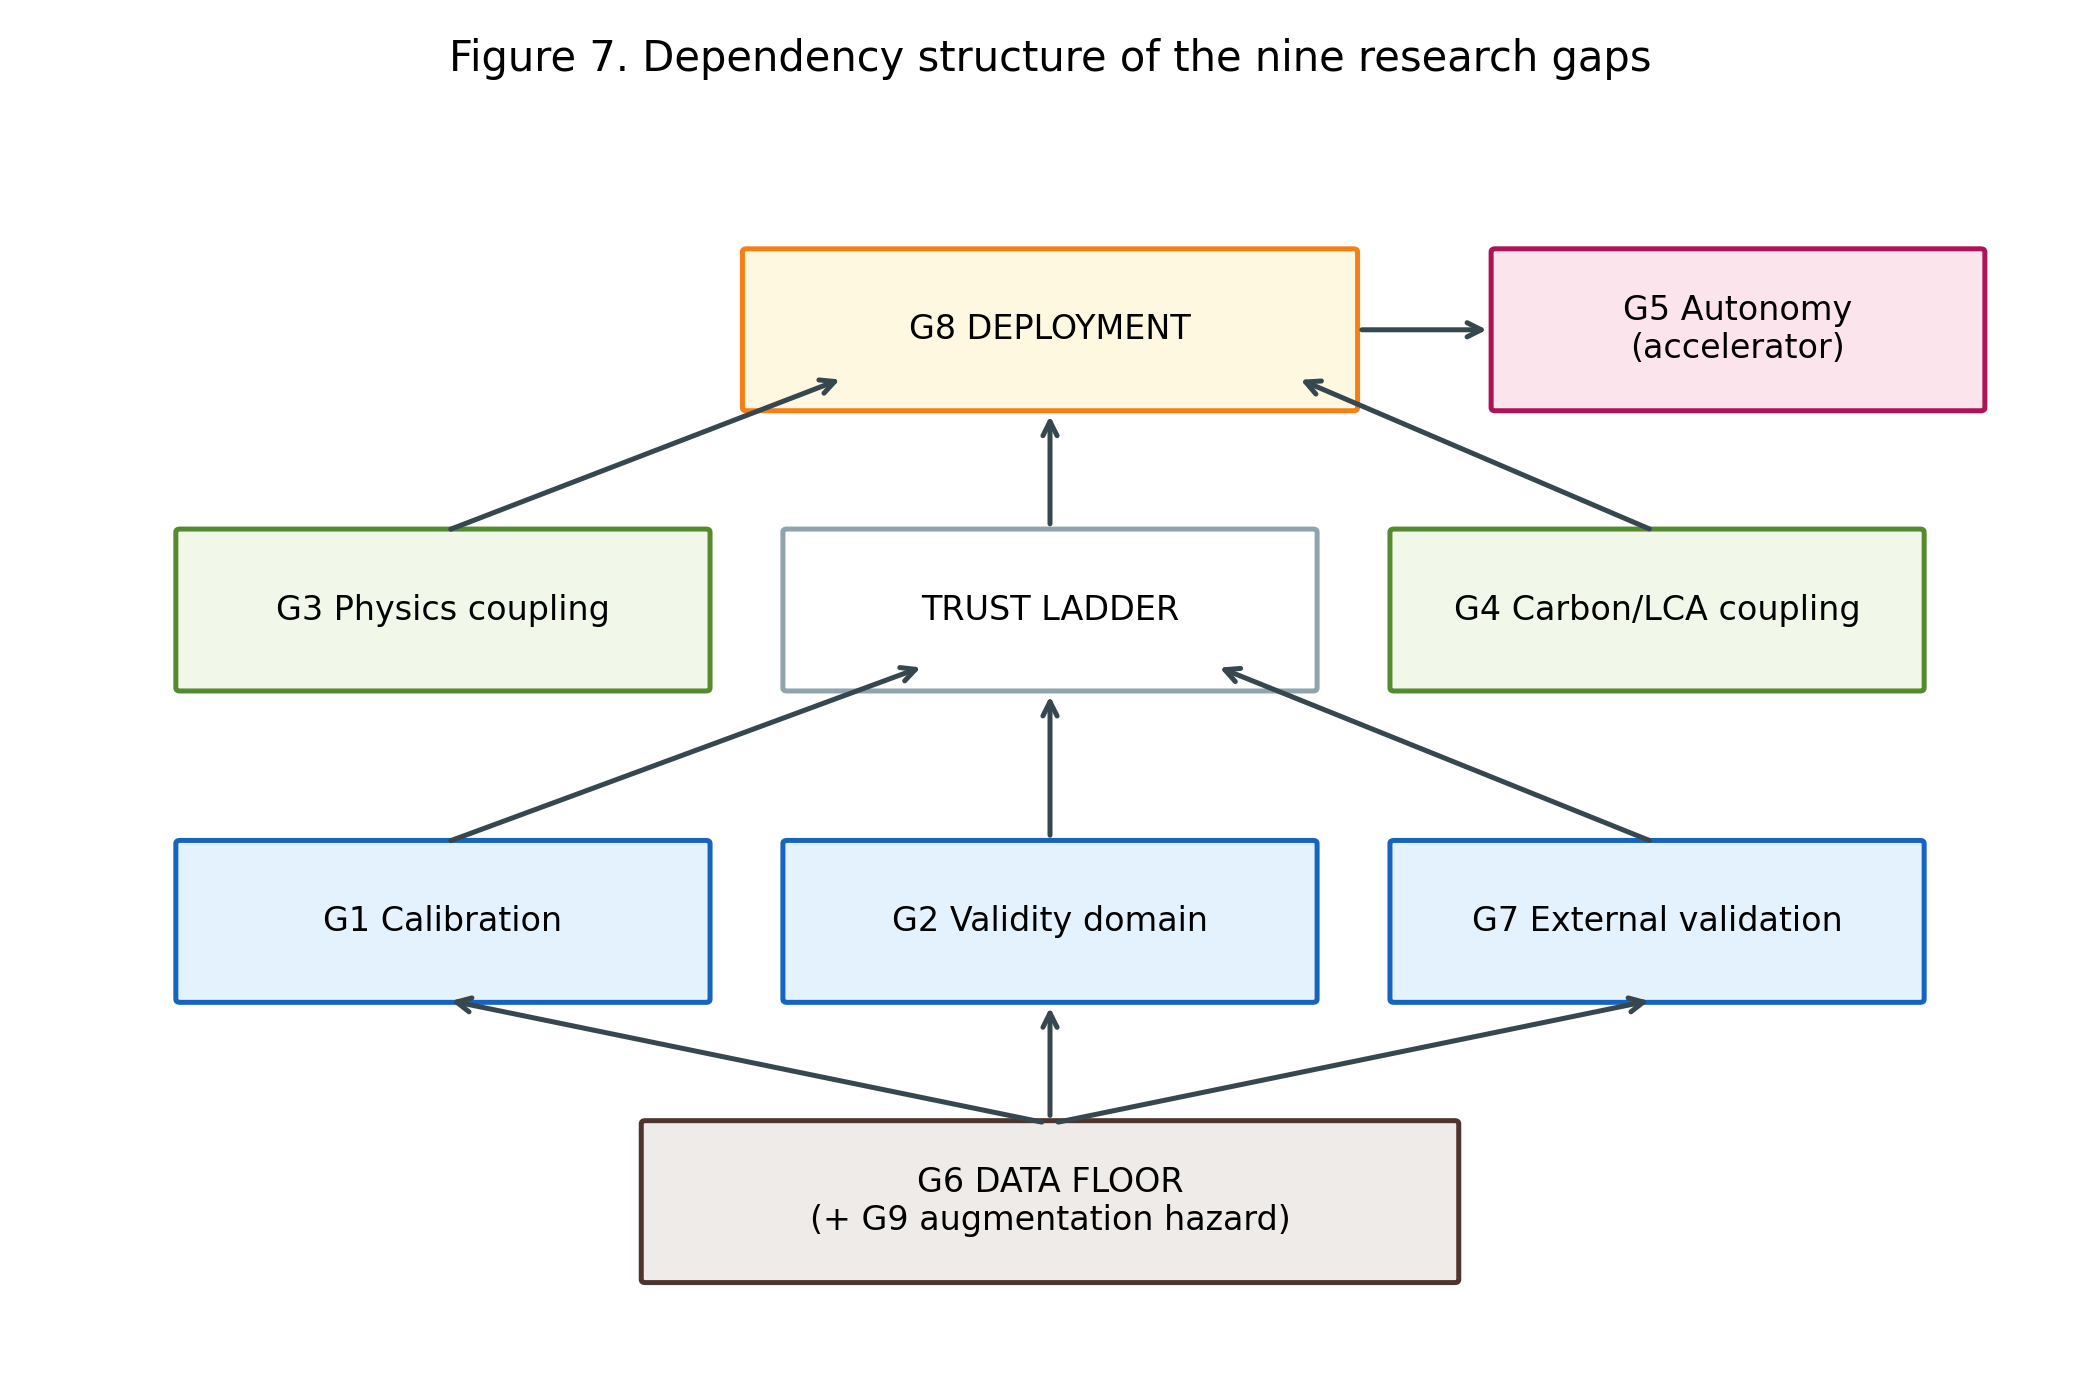
\includegraphics[width=0.95\textwidth]{Fig7.png}
\caption{Dependency structure of the nine research gaps}\label{fig7}
\end{figure}

\section{A Clean-Technology Roadmap: From Honest Models to Closed Loops}

The gaps of Section 19 are ordered by dependency --- data floor, trust ladder, physics and carbon couplings, autonomy accelerator, deployment superstructure --- and the roadmap inherits that order. Its stages are indicative horizons (immediate, 0--2 years; emerging, 2--5; frontier, 5--10) with a deployment-and-governance track running in parallel from the outset, because institutional change is the slowest component and, for a clean-technology outcome, the decisive one. Every item names its gap and its acceptance test (Table 7; Figure 8).

\subsection{Immediate priorities: make existing models honest}

Nothing in this tier requires a new laboratory. \textbf{(I1)} A FAIR community benchmark --- provenance-tracked, duplicate-audited, leakage-safe fixed splits, oxide-composition and environmental-inventory fields --- for which this review's released corpus is an explicit seed; done when three independent groups report on identical splits (G6). \textbf{(I2)} Calibration by default: conformal prediction intervals and coverage reporting retrofitted to standard pipelines, a practice already demonstrated on geopolymer data at trivial cost; done when coverage metrics appear beside R$^2$ as a reviewing norm (G1). \textbf{(I3)} Applicability-domain discipline imported from cheminformatics: group-aware splits, leave-one-source/precursor-out designs, validity-domain declarations, and degradation ladders from cross-validation to prospective test (G2, G7). \textbf{(I4)} Terminology discipline: the Type I--V physics-integration scale and the simulated-versus-physical adaptive labels adopted in reporting, so that claims remain auditable and the $\sim$50\% inflation rate measurably falls (G3, G5). \textbf{(I5)} Time-split meta-validation --- train on pre-2024 literature, test on the 2024--2026 flood --- executable immediately from published data and yielding the field's first forward-error estimate (G7).

\subsection{Emerging priorities: couple the models to chemistry and carbon}

\textbf{(E1)} Physics-constrained surrogates inside design loops: the verified frontier's three mechanisms --- thermodynamic hybrids, knowledge-graph guidance, embedded constraints --- combined (no study yet joins two) and moved from prediction into NSGA-II and Bayesian-optimization search, with constraint-violation audits and ablations isolating the physics contribution (G3). \textbf{(E2)} ML--LCA integration with uncertainty: regionalized inventories for dominant precursors and activators; emission-factor uncertainty propagated into Pareto fronts; ISO-consistent boundaries as the entry condition for "low-carbon" claims --- raising the current $\approx$0.3\% ISO-grade share by an order of magnitude would still leave it a minority practice (G4). \textbf{(E3)} The field's first cross-laboratory round-robin: one blind mix set, every willing published model, results public --- converting Section 15's unknown real-world error into a number (G2, G7). \textbf{(E4)} Early-age-updating models standardized as loop enablers, breaking the 28-day tempo barrier that currently forecloses adaptive work (G5, G1). \textbf{(E5)} Augmentation adjudication on the shared benchmark, with real-only test sets and physics checks, resolving Section 18's sharpest contradiction (G9).

\subsection{Frontier opportunities: close the loop, then scale it}

\textbf{(F1)} The first geopolymer self-driving laboratory. The entry point is argued, not assumed: one-part dry-mix formulations remove activator-solution handling, the corpus's most robot-hostile step; early-age surrogates (E4) fix tempo; calibrated acquisition (I2) supplies trustworthy exploration. Minimal credible demonstration: at least two consecutive physical propose--synthesize--test--update cycles with declining, calibrated uncertainty --- a result that would be publishable in itself and would move the trajectory's terminal stage from empty to inaugurated (G5). \textbf{(F2)} Digital twins of curing and durability evolution, assembled from ingredients the corpus already holds --- acoustic-emission staging, PINN transport parameters, posterior-updating strength models --- validated on a pilot element against measured service-life indicators. \textbf{(F3)} Language-model and agentic support systems, grounded in the two 2026 entry points (LLM-built knowledge graphs; tabular foundation models), deployed first where hallucination risk is auditable: literature-to-inventory extraction feeding E2, and protocol drafting for F1. No autonomous-agent claims are warranted until F1-class loops exist. \textbf{(F4)} Transferable foundation models for waste-derived binders: pre-trained across precursor chemistries, fine-tuned to local waste streams, certified by out-of-range performance bounds per deployment region (G2, G6).

\subsection{Deployment and governance: the parallel track that decides the outcome}

\textbf{(D1)} Performance-based acceptance protocols that consume model outputs as such --- predicted property, declared coverage, conformity-testing plan --- with the acceptance test being one AI-designed AAM mix approved at pilot scale (G8). \textbf{(D2)} Digital material passports binding provenance, oxide composition, LCA inventory, prediction intervals, and validity domain to each mix. \textbf{(D3)} A demonstration ladder from precast elements (low regulatory friction) through non-structural to structural pilots, each step publishing its model-versus-reality audit. Five governance levers support the track: a reporting checklist for AI-in-construction-materials studies, for which this review's scorecard is a working draft; an LCA-disclosure norm for sustainability claims, a lever a journal such as this one could pull directly; engagement of RILEM/ASTM/EN committees on model-based evidence, not detected in any of the 677 studies; community stewardship of the benchmark; and provenance integrity, including retraction propagation into compiled datasets --- a mechanism whose absence this review documented first-hand.

\subsection{The roadmap in one sentence}

Honest models first, chemistry- and carbon-coupled models second, closed loops third --- with deployment and governance advancing in parallel from day one, because they are slowest, and because a prediction that never leaves the laboratory decarbonizes nothing.

\begin{figure}[htbp]
\centering
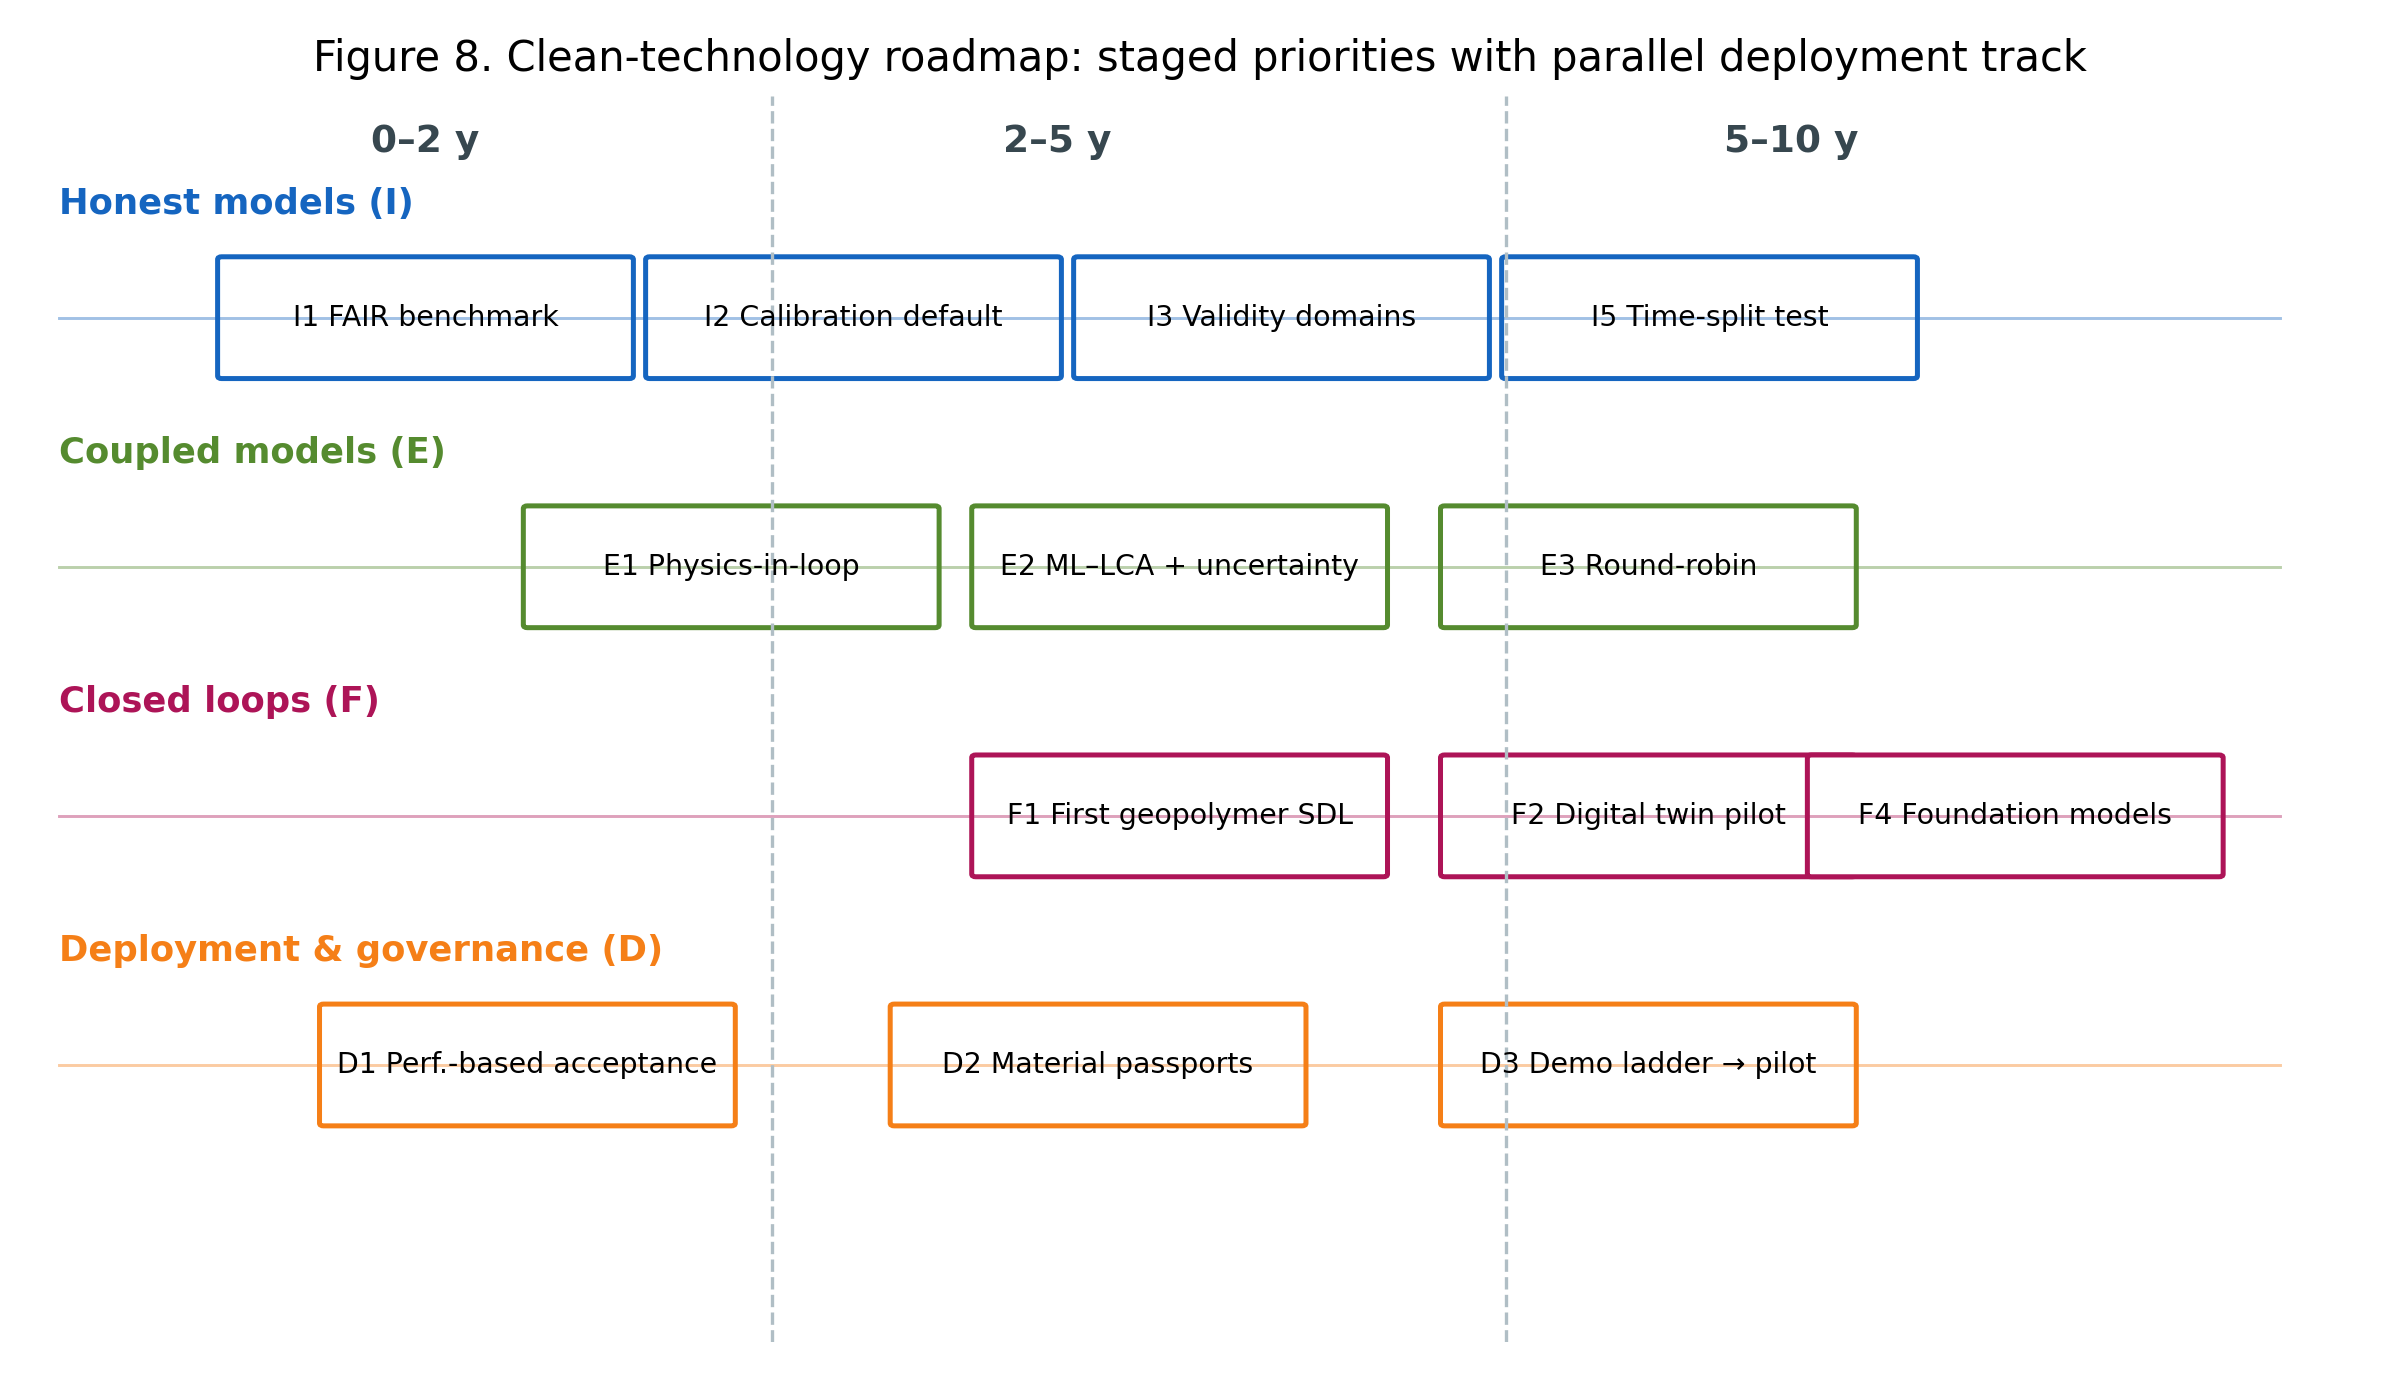
\includegraphics[width=0.95\textwidth]{Fig8.png}
\caption{The clean-technology roadmap with parallel deployment and governance track}\label{fig8}
\end{figure}

{\footnotesize
\begin{longtable}{llp{0.426\textwidth}lp{0.324\textwidth}}
\caption{The staged clean-technology roadmap: items, horizons, dependencies, and validation requirements}\\
\toprule
ID & Horizon & Priority & Gap & Acceptance test \\
\midrule
\endfirsthead
\toprule
ID & Horizon & Priority & Gap & Acceptance test \\
\midrule
\endhead
\bottomrule
\endfoot
I1 & 0-2y & FAIR benchmark (seeded by this artifact) & G6 & 3 groups on identical splits \\
I2 & 0-2y & Calibration by default (conformal) & G1 & coverage metrics beside R2 \\
I3 & 0-2y & Applicability-domain reporting & G2,G7 & validity domain declared per claim \\
I4 & 0-2y & Terminology discipline (Type I-V; sim/physical) & G3,G5 & claim inflation falls measurably \\
I5 & 0-2y & Time-split meta-validation & G7 & forward-error estimate published \\
E1 & 2-5y & Physics-constrained surrogates in design loops & G3 & constraint-violation audit + ablation \\
E2 & 2-5y & ML-LCA with factor-uncertainty propagation & G4 & ISO-consistent boundaries on claims \\
E3 & 2-5y & Cross-laboratory round-robin & G2,G7 & public blind-set results \\
E4 & 2-5y & Early-age updating as loop enabler & G5,G1 & validated qualification acceleration \\
E5 & 2-5y & Augmentation adjudication & G9,G6 & real-only-test parity shown \\
F1 & 5-10y & First geopolymer self-driving lab (one-part entry) & G5 & $>$=2 physical closed cycles, calibrated \\
F2 & 5-10y & Curing/durability digital twin pilot & G5,G3 & twin-vs-measured on pilot element \\
F3 & 5-10y & LLM/agentic support (prospective) & G5,G4,G6 & audited agent-extracted inventories \\
F4 & 5-10y & Transferable foundation models & G2,G6 & certified out-of-range bounds \\
D1 & parallel & Performance-based acceptance protocols & G8,G1 & one AI-designed mix approved (pilot) \\
D2 & parallel & Digital material passports & G8,G4,G6 & passport schema in a procurement pilot \\
D3 & parallel & Demonstration ladder w/ model audits & G8,G7 & published model-vs-reality trail \\
\end{longtable}}

\section{Limitations and Threats to Validity of This Review}

The audits this review applies to its corpus apply equally to itself; this section is written to that standard.

\textbf{Coverage.} Scopus served as the sole primary citation index: no Web of Science Core Collection entitlement was available. The SpringerLink supplement was originally harvested only to relevance depth (top 20 of 950 full-text matches); to convert this open-ended weakness into a bounded one, a random sample of 50 of the 930 unharvested records was subsequently screened against the eligibility criteria, and the estimated yield of additional eligible studies is reported in Supplementary Note S7 --- small relative to the corpus, because SpringerLink full-text matching inflates counts with studies that merely cite geopolymer work, and because eligible Springer-published studies reach the pool through Scopus indexing. The multi-source design (Scopus, ScienceDirect, Crossref, SpringerLink, IEEE Xplore) and the 894-record identification pool mitigate single-index bias, but studies indexed exclusively in WoS may be missed. English-only inclusion excludes a Chinese- and Persian-language applied literature of unknown but probably non-trivial size. Snowballing and a pre-submission delta search remain to be executed and will be reported as PRISMA amendments.

\textbf{Duplicate handling.} The corpus merge missed 52 abbreviated-title duplicate reports that were caught only by a post-freeze audit (Section 2.6); statistics published before that audit would have been computed on inflated denominators. The audit, its decision rules, and its pair-level evidence are released, and all statistics in this manuscript use the deduplicated n = 677.

\textbf{Screening and human factors.} Although every record was independently verified by one of two co-authors (primary + 1 design, with a 50-record doubly-verified calibration block; Section 2.3) and all disagreements adjudicated by consensus, verifier agreement was imperfect ($\kappa$ = 0.830 and 0.689 pre-resolution), one verifier's systematic misreading of a single tag accounted for a third of his disagreements, and post-consensus agreement is by construction not an independent check. The screening ledger is released so that any decision can be re-examined.

\textbf{Coding depth and reliability.} The corpus-wide statistics that anchor Sections 5--15 derive from title--abstract--keyword coding, verified by full-template extraction only for the deep tier and three cluster audits. Two independent blind recodes of a random 70-study sample --- one by a human co-author, one procedural (Table S9) --- quantify the coding's reliability per axis: the combined prediction-plus-optimization share, the Types I--II physics mass, and the reliability-side scorecard flags (calibration, uncertainty, reproducibility) recode at 93--100\% agreement under both, while the prediction-versus-optimization split (the optimization label absorbs metaheuristic tuning --- a finding both recodes reach independently), the Type I-versus-II boundary, the environmental-none judgment, and the explainability flag are criterion-sensitive and are therefore reported as indicative figures or bounds in the text. In each case the criterion drift runs in the direction that \emph{strengthens} the review's conclusions: design search smaller than labelled (10--17\% versus 34.0\%), environmental quantification rarer (both recodes reclassify toward "none"), and explainability more liberally credited than any reliability practice (it is the sole flag on which the three passes span a wide band, 19--48\% at sample level, while calibration and reproducibility recode identically under all three). The recodes also yielded a residual screening-error estimate: the human coder declared 3 of 70 sampled records ineligible (4.3\% [1.5--11.9]; two out-of-scope, one review), a strict subset of the six flagged procedurally (8.6\% [4.0--17.5]) --- all six flagged individually in the released corpus file. The effect of this residual is quantified directly: recomputing every headline proportion on the eligible subset (n = 671, the six flagged records excluded) moves no figure by more than 0.3 percentage points --- no-trust 60.1\% $\rightarrow$ 59.9\%, environmental-none 44.8\% $\rightarrow$ 44.9\%, prediction-plus-optimization 95.7\% $\rightarrow$ 96.0\% --- because the ineligible records are few and their codes are near the corpus modes (Supplementary Table S9, sensitivity panel). The residual does not touch the zero-claims or the cluster audits, which were full-text verified. Abstract-level coding also systematically \emph{under-detects} practices reported only in full text --- external validation and artifact availability above all --- so the trust-practice percentages reported here are best read as lower bounds, and the qualitative asymmetry (explainability versus reliability) is more secure than any individual figure; this is also why every zero claim in Sections 8--16 states its detection basis, and why the strongest zeros are those backed by dedicated search arms rather than coding absence. Conversely, physics-integration audits grade claims against abstracts and methods summaries; four claims remained unverifiable and are counted as neither confirmed nor deflated. The tiered design, pre-registered before extraction, trades exhaustive depth for auditability at scale; the released artifact permits anyone to deepen any cell of it.

\textbf{Exemplar concentration.} The manuscript's named best-practice exemplars trace to a small number of author groups --- the conformal-calibration and inverse-design exemplars in particular come from one overlapping cluster (Section~8.3), which supplies evidence for the roadmap's highest-priority item (I2). This concentration is a property of the field (calibrated uncertainty currently is the practice of one or two teams), but it means single-group idiosyncrasies could color what this review presents as best practice; the roadmap's validation requirements are stated so that any group can satisfy them independently.

\textbf{Analytic choices.} The taxonomy's axes and priority rules, the scorecard's dimensions, and the environmental evidentiary ladder are constructed instruments; other reasonable constructions exist. Their defense is procedural --- fixed before coding, applied conservatively, released in full --- rather than uniqueness. The invalid-comparison rule prevents this review from ranking model performance across studies, which readers seeking "the best algorithm" may experience as a refusal; it is one, and it is deliberate.

\textbf{Team composition.} No author is a certified LCA practitioner. Section 11 accordingly \emph{audits} the field's life-cycle practice against ISO 14040/44 criteria --- an assessment-methodology task --- and refrains from performing or adjudicating LCAs; the environmental-claims analysis was led by the team's materials-sustainability expertise and is fully traceable to the released audit table. Relatedly, the first and third authors of this review co-authored one primary study captured by the search; it is named with full citation in the Competing Interests statement, entered the corpus on identical criteria to all others, is not among the manuscript's cited exemplars, and received no analytical prominence --- claims verifiable from the released per-record codes. By coincidence of the worksheet split, its assigned screening verifier was also one of its authors; we disclose this rather than obscure it, and note that the record's eligibility is mechanically checkable from its published metadata.

\textbf{Temporal validity.} The corpus freezes at August 2026 in a field where 71\% of the evidence postdates January 2024. The quantitative shares reported here will age quickly; the audit instruments, gap framework, and roadmap are designed to outlive them, and the released artifact allows the numbers to be recomputed as the field moves.

\section{Conclusions}

This review set out to test a hypothesis: that AI applications in geopolymer research remain predominantly prediction-centric, constrained by fragmented data, inconsistent validation, weak physical and environmental integration, and negligible movement toward adaptive or autonomous discovery. Across 677 systematically selected unique studies, the hypothesis is \textbf{supported with one substantive revision}. The field is no longer merely prediction-centric --- a genuine design-search cluster, roughly 10--17\% of the corpus by independent recount (up to a third under liberal labeling; Table S9), now searches design spaces through optimization and inverse methods, an advance the original framing understates. But the search runs on uncalibrated, envelope-bound models (calibration 1.3\%, external validation 4.0\%), over recycled datasets whose provenance is invisible, guided by physics that is claimed twice as often as it is practiced (verified integration: nine studies, 1.3\%), toward environmental objectives that are almost never assessed (ISO-grade LCA $\approx$0.3\%) --- and no closed physical experimental loop was detected anywhere in it.

The constructive reading is equally supported: every deficiency identified here is answered by demonstrated best practice \emph{within the corpus itself} --- conformal calibration, applicability-domain declaration, thermodynamic and constraint-embedded modeling, boundary-explicit LCA, early-age posterior updating. The field's problem is not capability but diffusion, and diffusion responds to infrastructure and norms. Hence the roadmap's order: a shared benchmark and honesty conventions now; chemistry- and carbon-coupled design next; the first closed loop after that; and acceptance frameworks --- performance-based approval, material passports, disclosure norms --- built in parallel throughout, because a model that never meets a standard decarbonizes nothing.

For Clean Technologies and Environmental Policy's readership the summary is this: artificial intelligence has made low-carbon geopolymers dramatically easier to \emph{predict} and has only begun to make them easier to \emph{trust, assess, and deploy}. The distance between those verbs is the research program this review has tried to specify --- gap by gap, with acceptance criteria --- and the released corpus, audits, and instruments are offered as its starting infrastructure.

\backmatter

\bmhead{Supplementary information}
Supplementary Materials accompany this article: Table S1 (PRISMA arithmetic reconciliation), Table S8 (Wilson 95\% confidence intervals for all reported proportions), Note S7 (SpringerLink unharvested-records sample screen), and Table S9 (independent coding-reliability recode).

\bmhead{Acknowledgments}
The authors thank the maintainers of the open databases and open-access publications on which this synthesis depends.

\section*{Declarations}

\bmhead{Funding}
The authors declare that no funds, grants, or other support were received during the preparation of this manuscript.

\bmhead{Competing interests}
Two authors of this review (V.N. and S.S.A.) are authors of one primary study captured by the systematic search: Nageshwaran V, Amritphale SS, Ezekiel S (2026) Interpretable machine learning for one-part fly-ash/slag geopolymer strength prediction: Toward multifunctional binder design, Materials 19:3347, \url{https://doi.org/10.3390/ma19153347} --- record CR9 in the released ledger. The study entered the corpus under criteria identical to all others. Because, by coincidence of the verification-worksheet split, both its primary screener and its assigned independent verifier are among its authors, we note that its eligibility is mechanically checkable from its published metadata (peer-reviewed journal article applying ML to a geopolymer system for a construction function), and its released per-record codes show it received no analytical prominence: standard-tier coding (Type I, prediction task, explainability flag only), not cited anywhere in this manuscript, and not among its exemplars. The authors have no other relevant financial or non-financial interests to disclose.

\bmhead{Data availability}
The complete research artifact --- screening ledger with per-record decision codes, the coded corpus (729 records, 677 unique studies, duplicates flagged), duplicate-audit evidence, cluster-audit tables (physics integration; carbon/LCA), extraction files, figures, tables, and analysis scripts --- is permanently archived at Zenodo (version v1.1, \url{https://doi.org/10.5281/zenodo.22319864}) and maintained at \url{https://github.com/vnageshwaran-de/geopolymer-ai-review-artifact} (release v1.1; repository private during review). The Zenodo record provides editors and reviewers direct access throughout review, with no request step required.

\bmhead{Author contributions}
VN: conceptualization, methodology, software, formal analysis, investigation, data curation, writing --- original draft, visualization. PB: validation (independent screening; blind coding-reliability recode, Supplementary Table S9; environmental-claims review), investigation, writing --- review and editing. SSA: validation (independent screening; geopolymer-science review), resources, writing --- review and editing, supervision. All authors read and approved the final manuscript, including the post-audit revision.

\bmhead{Ethics approval}
Not applicable; this study involved no human participants or animals.

\bibliography{sn-bibliography}

\end{document}
